              %******************************************%
              %                                          %
              % Modello di tesi di laurea o di dottorato %
              %            di Lorenzo Pantieri           %
              %                                          %
              %                © 2013-2017               %
              %                                          %
              %******************************************%
       

% I seguenti commenti speciali impostano:
% 1. utf8 come codifica di input,
% 2. PDFLaTeX come motore di composizione;
% 3. Tesi.tex come documento principale;
% 4. il controllo ortografico italiano per l'editor.

% !TEX encoding = UTF-8 Unicode
% !TEX TS-program = pdflatex
% !TEX root = Tesi.tex
% !TEX spellcheck = it-IT

\documentclass[11pt,%                      % corpo del font principale
               a4paper,%                   % carta A4
               twoside,openright,%         % fronte-retro
%              oneside,openany,%           % solo fronte
               titlepage,%                 % frontespizio
               headinclude,,footinclude,%  % testatina e piede di pagina
               BCOR5mm,%                   % rilegatura di 5 mm
               cleardoublepage=empty,%     % pagine vuote senza testatina e piede di pagina
               captions=tableheading,%     % didascalie in cima alle tabelle
               ]{scrreprt}                 % classe report di KOMA-Script;
               
\usepackage[T1]{fontenc}                   % codifica dei font:
                                           % NOTA BENE! richiede una distribuzione *completa* di LaTeX,
                                           % per esempio TeXLive o MiKTeX *complete*

\usepackage[utf8]{inputenc}                % codifica di input; anche [latin1] va bene
                                           % NOTA BENE! va accordata con le preferenze dell'editor

\usepackage[english,italian]{babel}        % per scrivere in italiano e in inglese;
                                           % l'ultima lingua (l'italiano) risulta predefinita

\usepackage[suftesi]{frontespizio}         % frontespizo
                                           % per includerlo nel documento bisogna:
                                           % 1. compilare una prima volta Tesi.tex;
                                           % 2. compilare a parte Tesi-frn.tex, generato dalla compilazione precedente;
                                           % 3. compilare ancora Tesi.tex. 

\usepackage{indentfirst}                   % rientra il primo capoverso di ogni sezione

\usepackage{graphicx}                      % immagini

\usepackage{listings}                      % codici

\usepackage[font=small]{quoting}           % citazioni

\usepackage{amsmath,amssymb,amsthm}        % matematica

\usepackage[italian]{varioref}             % riferimenti completi della pagina

\usepackage{tabularx}                      % tabelle di larghezza prefissata

\usepackage[autostyle,italian=guillemets]{csquotes} % virgolette ottimizzate per biblatex

\usepackage[style=philosophy-modern,hyperref,square,backend=biber]{biblatex}
                                           % eccellente pacchetto per la bibliografia;
                                           % produce uno stile di citazione autore-anno; 
                                           % lo stile "numeric-comp" produce riferimenti numerici;
                                           % NOTA BENE! bisogna che il proprio editor sia configurato per biber
                                          
\addbibresource{Bibliografia.bib}          % database di biblatex 
                                          
\usepackage{subfig}                        % sottofigure, sottotabelle

\usepackage{lipsum}                        % testo fittizio

\usepackage{eurosym}                       % simbolo dell'euro

\usepackage[eulerchapternumbers,%          % numeri dei capitoli nel font Euler
            subfig,%                       % se si usa il pacchetto subfig
            beramono,%                     % Bera Mono come font a spaziatura fissa
            eulermath,%                    % AMS Euler come font per la matematica
            pdfspacing,%                   % migliora il riempimento di riga
            listings,%                     % codici
%           parts,%                        % da decommentare in un documento diviso in parti
            ]{classicthesis}               % stile ClassicThesis

\usepackage{arsclassica}                   % modifica l'aspetto di ClassicThesis

%*********************************************************************************
% impostazioni-tesi.tex
% di Lorenzo Pantieri (2013-2016)
% file che contiene le impostazioni della tesi
%*********************************************************************************


%*********************************************************************************
% Comandi personali
%*******************************************************
\newcommand{\myName}{Marco De Martino}                           % autore
\newcommand{\myTitle}{appunti sul marmo} % titolo
\newcommand{\myDegree}{Tesi di laurea}                           % tipo di tesi
\newcommand{\myUni}{Conservatorio di Musica S. Cecilia di Roma}       % universit�
\newcommand{\myFaculty}{Musica Elettronica}        % facolt\'a
\newcommand{\myDepartment}{Nuove Tecnologie}             % dipartimento
\newcommand{\myProf}{Prof.~Michelangelo Lupone}          % relatore
\newcommand{\myOtherProf}{Prof.~Nicola Bernardini}                  % correlatore (se presente)
\newcommand{\myLocation}{Roma}                                 % dove
\newcommand{\myTime}{Aprile 2017}                               % quando



%*********************************************************************************
% Impostazioni di amsmath, amssymb, amsthm
%*********************************************************************************

% comandi per gli insiemi numerici (serve il pacchetto amssymb)
\newcommand{\numberset}{\mathbb} 
\newcommand{\N}{\numberset{N}} 
\newcommand{\R}{\numberset{R}} 

% un ambiente per i sistemi
\newenvironment{sistema}%
  {\left\lbrace\begin{array}{@{}l@{}}}%
  {\end{array}\right.}

% definizioni (serve il pacchetto amsthm)
\theoremstyle{definition} 
\newtheorem{definizione}{Definizione}

% teoremi, leggi e decreti (serve il pacchetto amsthm)
\theoremstyle{plain} 
\newtheorem{teorema}{Teorema}
\newtheorem{legge}{Legge}
\newtheorem{decreto}[legge]{Decreto}
\newtheorem{murphy}{Murphy}[section]



%*********************************************************************************
% Impostazioni di biblatex
%*********************************************************************************
\defbibheading{bibliography}{%
\cleardoublepage
\manualmark
\phantomsection 
\addcontentsline{toc}{chapter}{\tocEntry{\bibname}}
\chapter*{\bibname\markboth{\spacedlowsmallcaps{\bibname}}
{\spacedlowsmallcaps{\bibname}}}}



%*********************************************************************************
% Impostazioni di listings
%*********************************************************************************
\lstset{language=[LaTeX]Tex,%C++,
    keywordstyle=\color{RoyalBlue},%\bfseries,
    basicstyle=\small\ttfamily,
    %identifierstyle=\color{NavyBlue},
    commentstyle=\color{Green}\ttfamily,
    stringstyle=\rmfamily,
    numbers=none,%left,%
    numberstyle=\scriptsize,%\tiny
    stepnumber=5,
    numbersep=8pt,
    showstringspaces=false,
    breaklines=true,
    frameround=ftff,
    frame=single
} 



%*********************************************************************************
% Impostazioni di hyperref (decommenta le seguenti righe se non carichi arsclassica)
%*********************************************************************************
%\hypersetup{%
%    hyperfootnotes=false,pdfpagelabels,
%    %draft,	% = elimina tutti i link (utile per stampe in bianco e nero)
%    colorlinks=true, linktocpage=true, pdfstartpage=1, pdfstartview=FitV,%
%    % decommenta la riga seguente per avere link in nero (per esempio per la stampa in bianco e nero)
%    %colorlinks=false, linktocpage=false, pdfborder={0 0 0}, pdfstartpage=1, pdfstartview=FitV,% 
%    breaklinks=true, pdfpagemode=UseNone, pageanchor=true, pdfpagemode=UseOutlines,%
%    plainpages=false, bookmarksnumbered, bookmarksopen=true, bookmarksopenlevel=1,%
%    hypertexnames=true, pdfhighlight=/O,%nesting=true,%frenchlinks,%
%    urlcolor=webbrown, linkcolor=RoyalBlue, citecolor=webgreen, %pagecolor=RoyalBlue,%
%    %urlcolor=Black, linkcolor=Black, citecolor=Black, %pagecolor=Black,%
%    pdftitle={\myTitle},%
%    pdfauthor={\textcopyright\ \myName, \myUni, \myFaculty},%
%    pdfsubject={},%
%    pdfkeywords={},%
%    pdfcreator={pdfLaTeX},%
%    pdfproducer={LaTeX with hyperref and ClassicThesis}%
%}



%*********************************************************************************
% Impostazioni di graphicx
%*********************************************************************************
\graphicspath{{Immagini/}} % cartella dove sono riposte le immagini



%*********************************************************************************
% Margini ottimizzati per l'A4
%*********************************************************************************
\areaset[current]{370pt}{750pt}
\setlength{\marginparwidth}{7em}
\setlength{\marginparsep}{2em}%



%*********************************************************************************
% Impostazioni di varioref
%*********************************************************************************
\makeatletter
\vref@addto\extrasitalian{%
   \def\reftextfaraway#1{a pagina~\pageref{#1}}%
}
\makeatother



%*********************************************************************************
% Altro
%*********************************************************************************

% [...] ;-)
\newcommand{\omissis}{[\dots\negthinspace]}

% eccezioni all'algoritmo di sillabazione
\hyphenation{Fortran ma-cro-istru-zio-ne nitro-idrossil-amminico}

% correzione di un bug di scrreprt nella numerazione delle figure
\renewcommand*{\figureformat}{%
  \figurename~\thefigure%
  %\autodot%
}
\renewcommand*{\tableformat}{%
  \tablename~\thetable%
  %\autodot%
}                  % file con le impostazioni personali

\usepackage{pdfpages}

\usepackage{musixtex}

\begin{document}
\pagestyle{scrheadings} 
\pagenumbering{roman}
%******************************************************************
% Materiale iniziale
%******************************************************************
% !TEX encoding = UTF-8
% !TEX TS-program = pdflatex
% !TEX root = ../Tesi.tex
% !TEX spellcheck = it-IT

%*******************************************************
% Frontespizio
%*******************************************************
\begin{frontespizio}
\Preambolo{\usepackage{iwona}} % riga da commentare se non si carica ArsClassica

\Universita{Conservatorio di Musica S. Cecilia di Roma}
\Logo{Sigillo}
\Facolta{Dipartimento di Nuove Tecnologie}
\Corso{Musica Elettronica}
\Annoaccademico{2015--2016}
\Titoletto{TRIENNIO DI I LIVELLO}
\Titolo{appunti sul marmo}
\Sottotitolo{sottotitolo}
\Candidato[2240TR]{Marco De Martino}
\Relatore{Giuseppe Silvi}
%\Relatore{Claudio Beccari}
%\Correlatore{Tommaso Gordini}
%\Correlatore{Ivan Valbusa}
\end{frontespizio}
%% !TEX encoding = UTF-8
% !TEX TS-program = pdflatex
% !TEX root = ../Tesi.tex
% !TEX spellcheck = it-IT

%*******************************************************
% Colophon
%*******************************************************
\clearpage
\phantomsection
\thispagestyle{empty}

\hfill

\vfill

%\noindent\myName: \textit{\myTitle,}
%\myDegree,
%\textcopyright\ \MakeTextLowercase{\myTime}.

\lipsum[2]
% !TEX encoding = UTF-8
% !TEX TS-program = pdflatex
% !TEX root = ../Tesi.tex
% !TEX spellcheck = it-IT

%*******************************************************
% Dedica
%*******************************************************
%\cleardoublepage
\phantomsection
\thispagestyle{empty}
\pdfbookmark{Dedica}{Dedica}

~

\vfill

\begin{flushright}
C’è gente che trova figure \\
nascoste nella carta da parati \\
o nelle nuvole. \\
A me succede lo stesso coi rumori. \\
Per essere più esatti, ho un vecchio phon \\
che appena si accende comincia a vibrare \\
e man mano \\
emette un lamento profondo. \\
E’ l’elica difettosa, o i cuscinetti a sfera, \\
non ne ho idea, \\
ma so che inizia a intonare una trenodia, \\
o meglio, a sussurrarla sottovoce. \\
Prima si avvertono solo suoni indistinti, \\
una folla che fugge, moto che si avvicinano, \\
ma facendo attenzione \\
appaiono via via urla, richiami. \\
Io mi concentro; una sera, addirittura, \\
sono arrivato a bruciarmi, tale è lo sforzo \\
per afferrare il groviglio, il nodo acustico \\
dell’asciugacapelli. \\
Perché il suo sferragliare non resta sempre uguale: \\
più dura, più si sciolgono gli intrecci \\
del fragore, le voci si distinguono. \\
Sento dialetti slavi, minacce, spesso spari: \\
un giorno sono rimasto ad ascoltarlo quasi dieci minuti \\
per seguire la fasi di un rastrellamento \\
in un lontano villaggio dei Balcani. \\
A volte ne esce uno squillo familiare, \\
credo che sia il telefono, spengo, \\
vado a rispondere, \\
ma non c’é mai nessuno: quei segnali, \\
si vede che provengono da un’altra parte, \\
sempre. \\
Se qualcuno ti chiama, non ci credere,\\
sarà un miraggio uditivo, un’impressione. \\
La verità è diversa: \\
mentre mi punto alla tempia quell’attrezzo \\
che sembra una pistola, \\
viene fuori il racconto di storie terribili, \\
fucilazioni, il pianto di bambini. \\
E’ come una confessione non richiesta, \\
una registrazione spedita per errore. \\
Che c’entro, io, con tutto questo sangue, \\
io che mi voglio solo asciugare la testa? \\
Ormai ci penso due volte, prima di adoperarlo, \\
prima di sprofondare in quell’orrore \\
e assistere impotente a certe scene. \\
Meglio bagnato, allora. \\
Mi verrà il torcicollo? Poco male \\ \medskip
--- Valerio Magrelli\footnote{Valerio Magrelli (Roma, 1957),  da Il sangue amaro (Einaudi, 2014)}    

\end{flushright}
% !TEX encoding = UTF-8
% !TEX TS-program = pdflatex
% !TEX root = ../Tesi.tex
% !TEX spellcheck = it-IT

%*******************************************************
% Dedica
%*******************************************************
%\cleardoublepage
\phantomsection
\thispagestyle{empty}

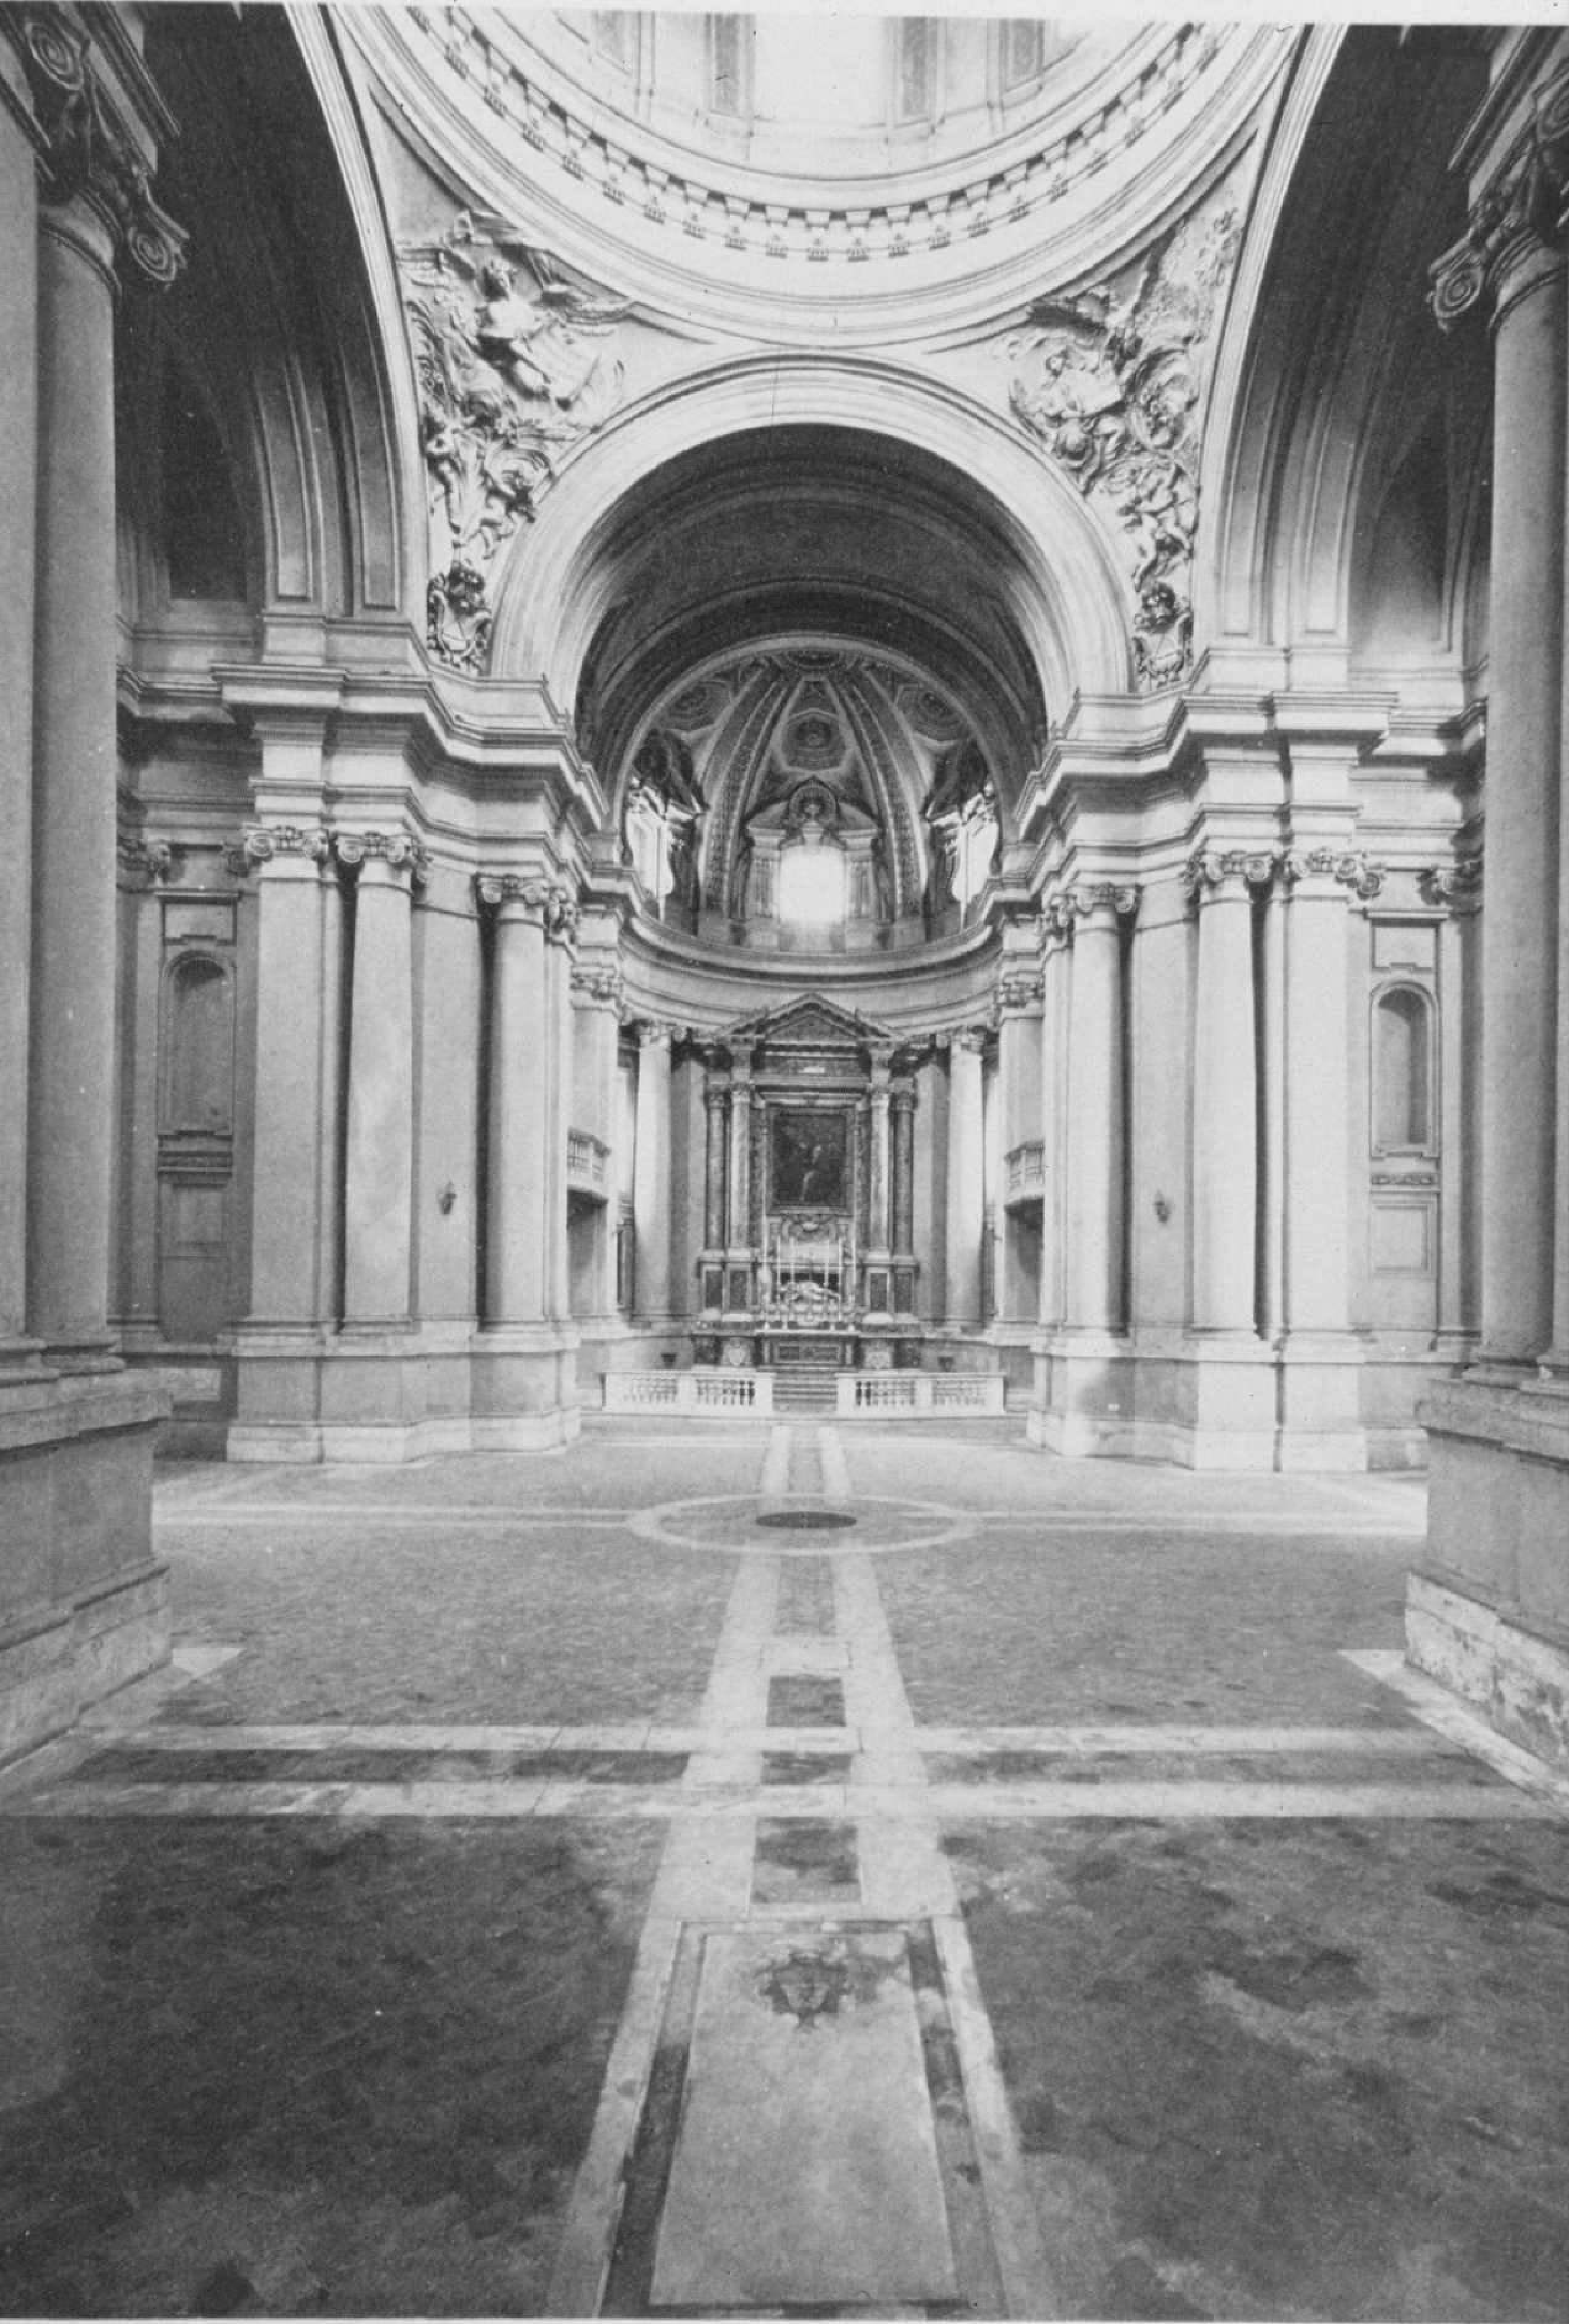
\includepdf[scale=1.1]{fotointerno.pdf}

%\fbox{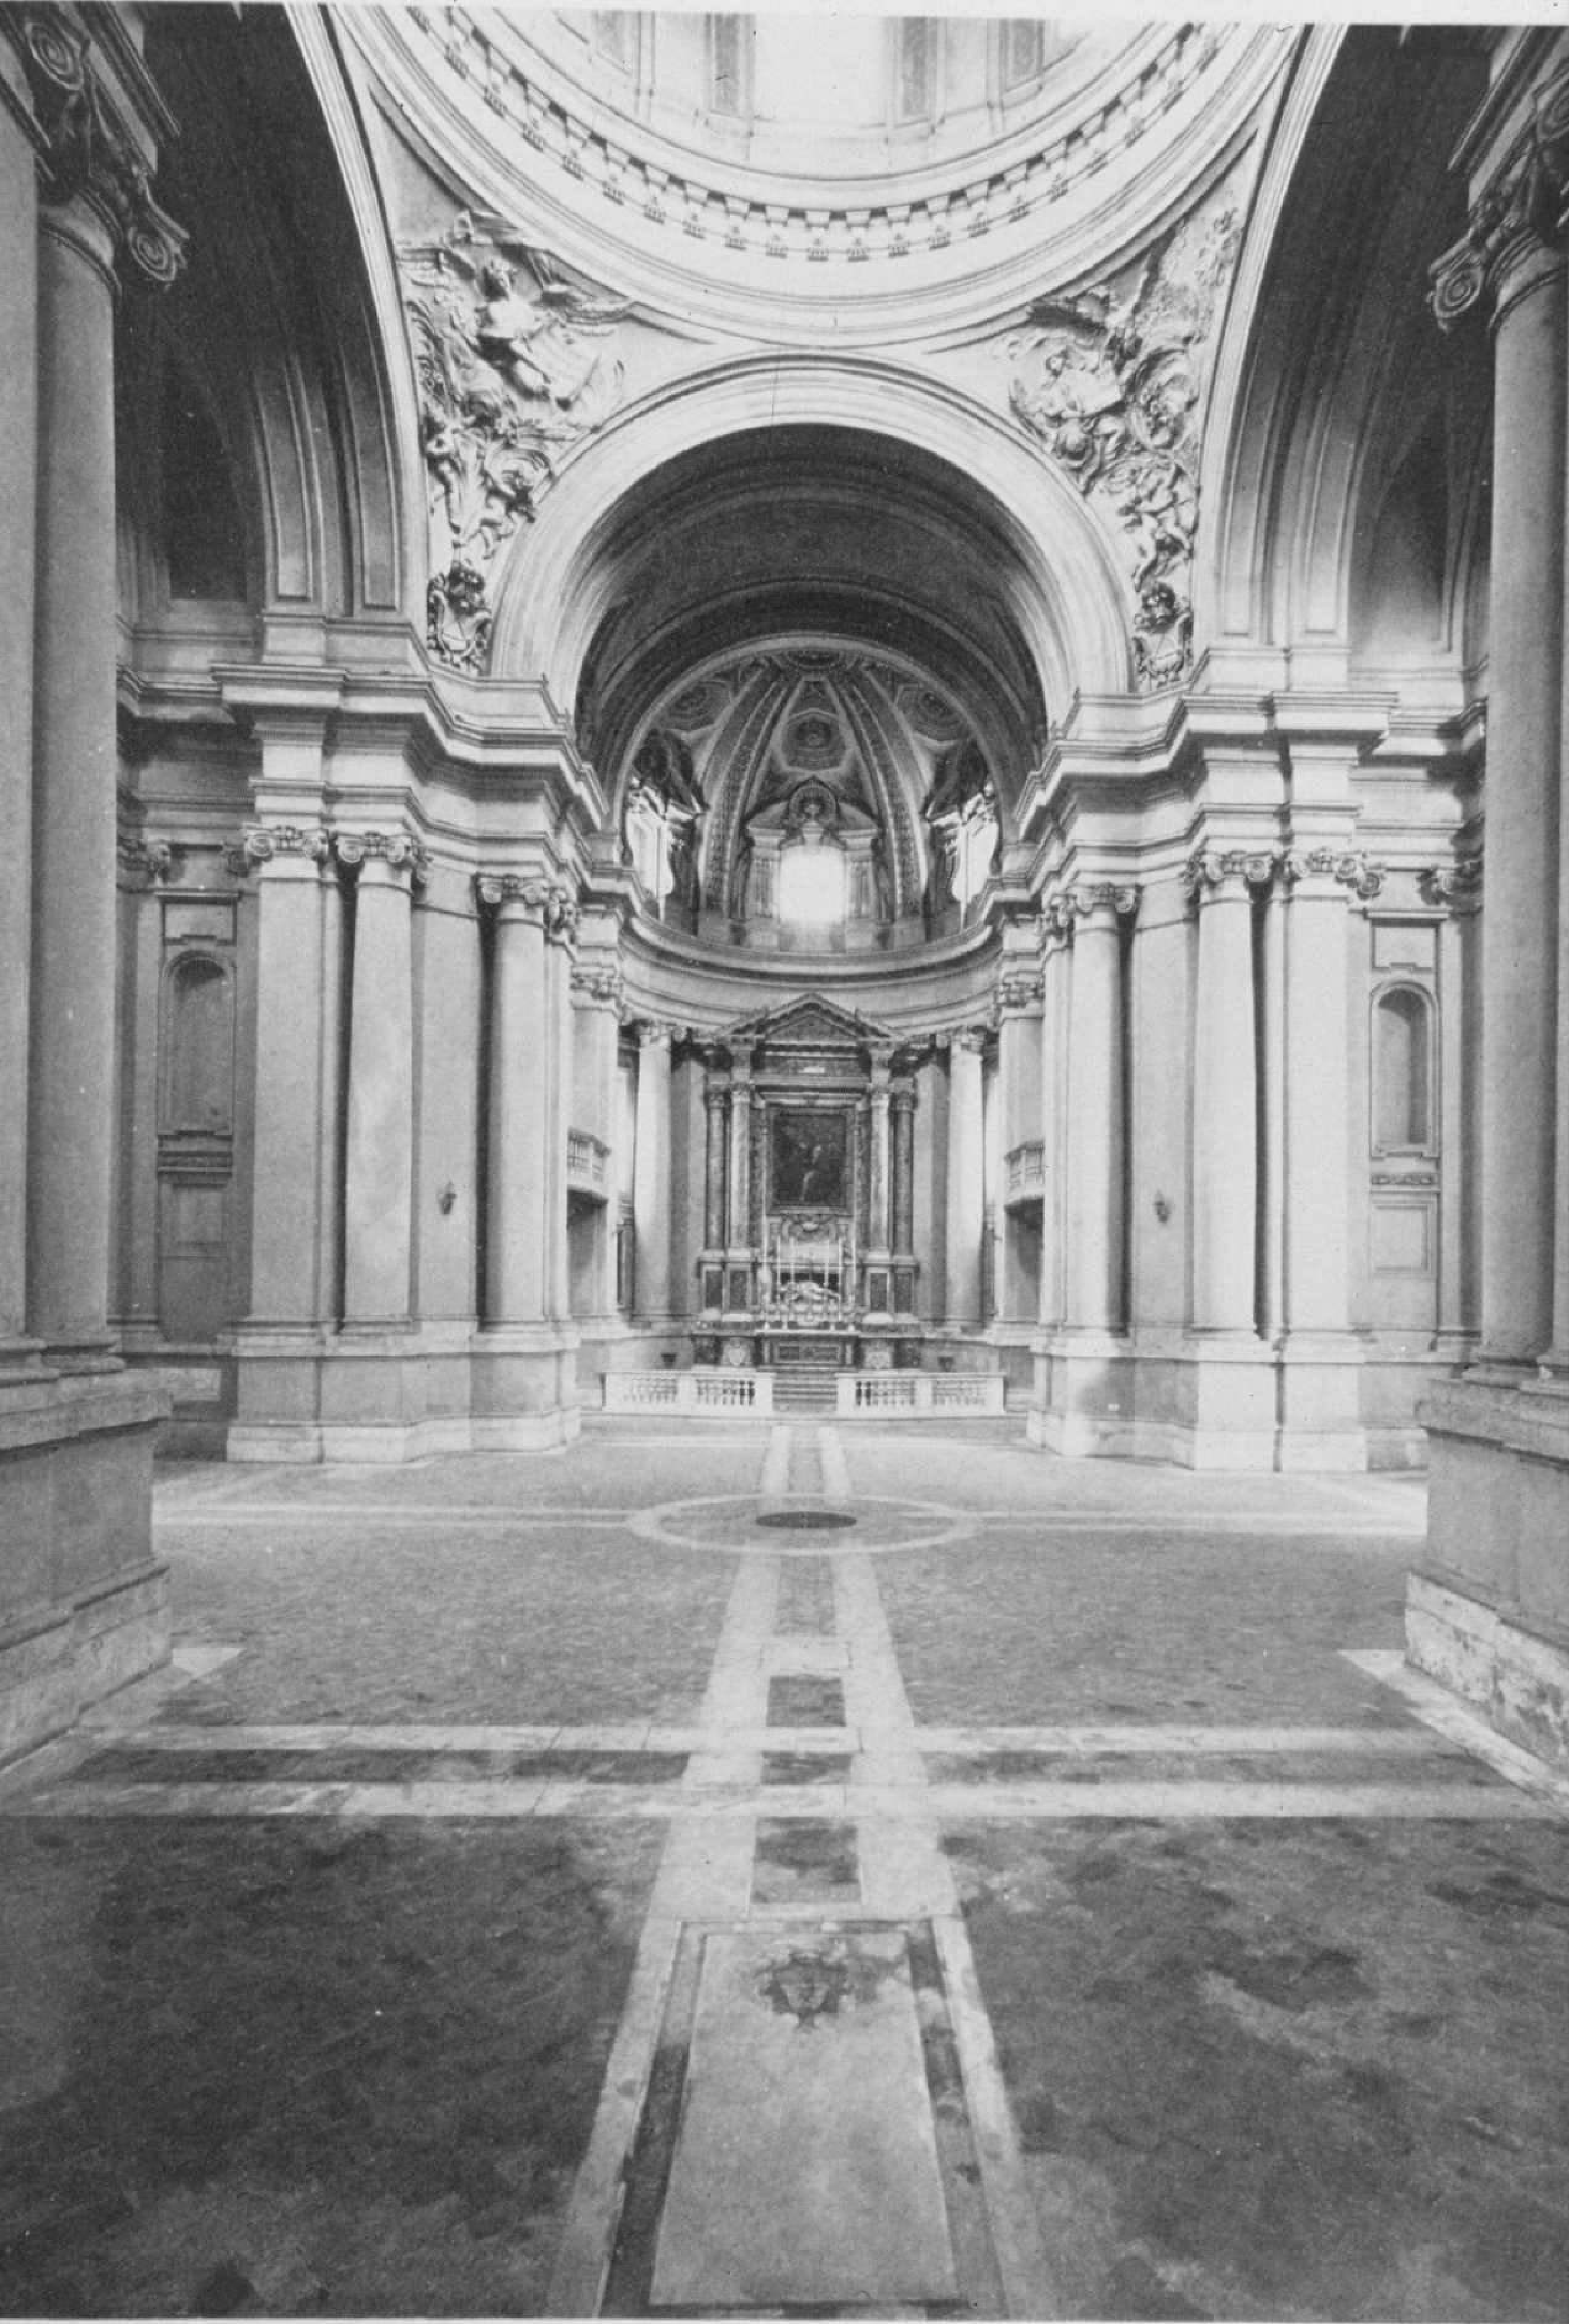
\includegraphics[page=1,scale=1.1]{fotointerno.pdf}}

%\begin{figure}
%\centering
%{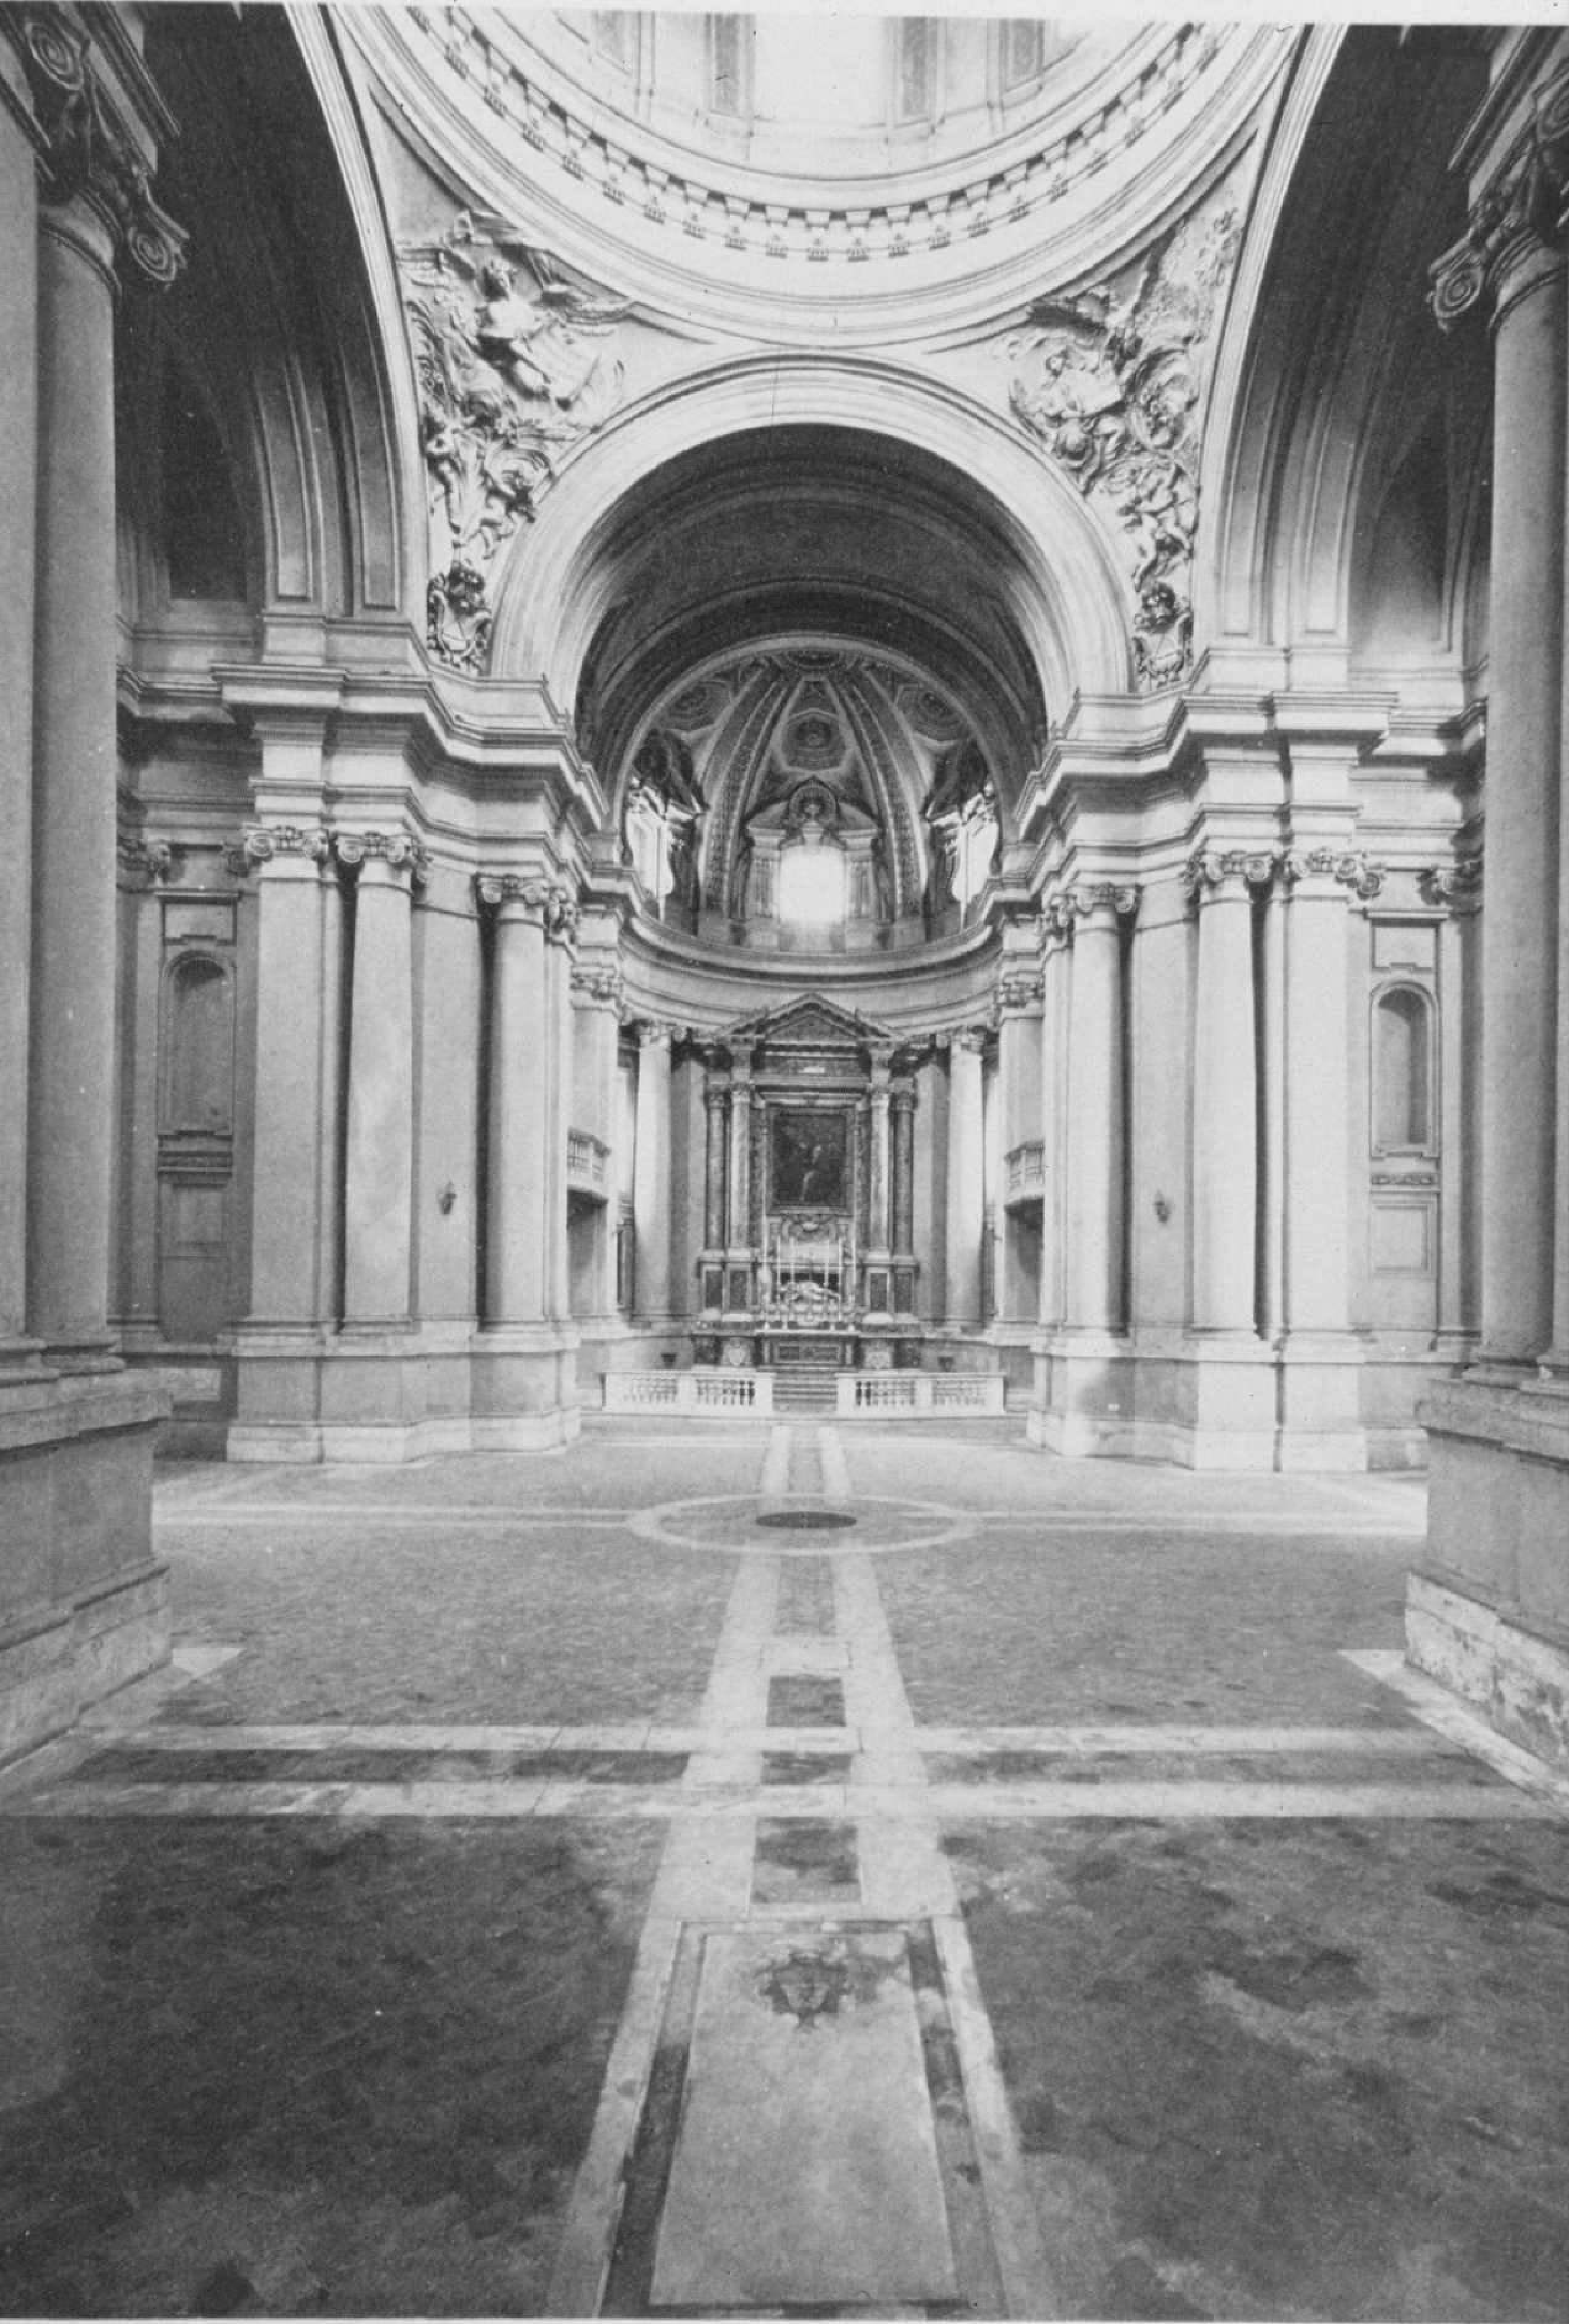
\includegraphics[width=.95\columnwidth]{fotointerno}}
%\caption[Pianta S. Luca]{Pianta S. Luca}
%\label{fig:tetratetra}
%\end{figure}
%% !TEX encoding = UTF-8
% !TEX TS-program = pdflatex
% !TEX root = ../Tesi.tex
% !TEX spellcheck = it-IT

%*******************************************************
% Dedica
%*******************************************************
%\cleardoublepage
\phantomsection
\thispagestyle{empty}
\pdfbookmark{Dedica}{Dedica}

~

\vfill

\begin{flushright}
C’è gente che trova figure \\
nascoste nella carta da parati \\
o nelle nuvole. \\
A me succede lo stesso coi rumori. \\
Per essere più esatti, ho un vecchio phon \\
che appena si accende comincia a vibrare \\
e man mano \\
emette un lamento profondo. \\
E’ l’elica difettosa, o i cuscinetti a sfera, \\
non ne ho idea, \\
ma so che inizia a intonare una trenodia, \\
o meglio, a sussurrarla sottovoce. \\
Prima si avvertono solo suoni indistinti, \\
una folla che fugge, moto che si avvicinano, \\
ma facendo attenzione \\
appaiono via via urla, richiami. \\
Io mi concentro; una sera, addirittura, \\
sono arrivato a bruciarmi, tale è lo sforzo \\
per afferrare il groviglio, il nodo acustico \\
dell’asciugacapelli. \\
Perché il suo sferragliare non resta sempre uguale: \\
più dura, più si sciolgono gli intrecci \\
del fragore, le voci si distinguono. \\
Sento dialetti slavi, minacce, spesso spari: \\
un giorno sono rimasto ad ascoltarlo quasi dieci minuti \\
per seguire la fasi di un rastrellamento \\
in un lontano villaggio dei Balcani. \\
A volte ne esce uno squillo familiare, \\
credo che sia il telefono, spengo, \\
vado a rispondere, \\
ma non c’é mai nessuno: quei segnali, \\
si vede che provengono da un’altra parte, \\
sempre. \\
Se qualcuno ti chiama, non ci credere,\\
sarà un miraggio uditivo, un’impressione. \\
La verità è diversa: \\
mentre mi punto alla tempia quell’attrezzo \\
che sembra una pistola, \\
viene fuori il racconto di storie terribili, \\
fucilazioni, il pianto di bambini. \\
E’ come una confessione non richiesta, \\
una registrazione spedita per errore. \\
Che c’entro, io, con tutto questo sangue, \\
io che mi voglio solo asciugare la testa? \\
Ormai ci penso due volte, prima di adoperarlo, \\
prima di sprofondare in quell’orrore \\
e assistere impotente a certe scene. \\
Meglio bagnato, allora. \\
Mi verrà il torcicollo? Poco male \\ \medskip
--- Valerio Magrelli\footnote{Valerio Magrelli (Roma, 1957),  da Il sangue amaro (Einaudi, 2014)}    

\end{flushright}
% !TEX encoding = UTF-8
% !TEX TS-program = pdflatex
% !TEX root = ../CME-III-ARTICOLO.tex
% !TEX spellcheck = it-IT

%*******************************************************
% Indici
%*******************************************************
\pdfbookmark{\contentsname}{tableofcontents}
\setcounter{tocdepth}{2}
\tableofcontents
\markboth{\spacedlowsmallcaps{\contentsname}}{\spacedlowsmallcaps{\contentsname}} 

%*******************************************************
% Elenco delle figure
%*******************************************************    
\phantomsection
\pdfbookmark{\listfigurename}{lof}
\listoffigures

%*******************************************************
% Elenco delle tabelle
%*******************************************************
\phantomsection
\pdfbookmark{\listtablename}{lot}
\listoftables
        

% !TEX encoding = UTF-8
% !TEX TS-program = pdflatex
% !TEX root = ../Articolo.tex
% !TEX spellcheck = it-IT

%*******************************************************
% Sommario+Abstract
%*******************************************************
\phantomsection
\pdfbookmark{Sommario}{Sommario}
\section*{Sommario}

\lipsum[1]

\selectlanguage{english}
\pdfbookmark{Abstract}{Abstract}
\section*{Abstract}

\lipsum[2]

\selectlanguage{italian}


% !TEX encoding = UTF-8
% !TEX TS-program = pdflatex
% !TEX root = ../Tesi.tex
% !TEX spellcheck = it-IT

%*******************************************************
% Ringraziamenti
%*******************************************************
\cleardoublepage
\phantomsection
\pdfbookmark{Ringraziamenti}{ringraziamenti}

\chapter*{Ringraziamenti}

\begin{flushright}{\slshape    
	Lorem ipsum dolor sit amet, consectetuer adipiscing elit. \\
	Ut purus elit, vestibulum ut, placerat ac, adipiscing vitae, felis. \\
	Curabitur dictum gravida mauris.} \\ \medskip
    --- Donald Ervin Knuth
\end{flushright}

\lipsum[1]

\bigskip
 
\noindent\textit{\myLocation, \MakeTextLowercase{\myTime}}
%% !TEX encoding = UTF-8
% !TEX TS-program = pdflatex
% !TEX root = ../Tesi.tex
% !TEX spellcheck = it-IT

%*******************************************************
% Introduzione
%*******************************************************
\cleardoublepage
\pdfbookmark{Introduzione}{introduzione}

\chapter*{Introduzione}

\lipsum[1]

Lorem ipsum dolor sit amet, consectetuer adipiscing elit.
\begin{description}
\item[{\hyperref[cap:lorem]{Il primo capitolo}}]
offre una visione d'insieme della storia di \LaTeX{} e ne vengono presentate le idee di fondo.
\item[{\hyperref[cap:ipsum]{Il secondo capitolo}}]
spiega le operazioni, veramente semplici, per installare \LaTeX{} sul proprio calcolatore.
\item[{\hyperref[cap:dolor]{L'appendice A}}] descrive  sinteticamente le principali norme tipografiche della lingua italiana, utili nella composizione di articoli, tesi o libri.
\end{description}

\lipsum[2]
\cleardoublepage
%******************************************************************
% Materiale principale
%******************************************************************
\pagenumbering{arabic}
% !TEX encoding = UTF-8
% !TEX TS-program = pdflatex
% !TEX root = ../Tesi.tex
% !TEX spellcheck = it-IT

%************************************************
\chapter{Introduzione allo logica dello spazio}
\label{cap:spazio}
%************************************************

\vfill

\begin{flushright}{\slshape
  …sì, per cui una chiesa barocca ha sotto di sé, \\
  accessibile, una chiesa romanica, \\
  sotto la chiesa romanica una basilica paleocristiana, \\
  poi si scende ancora e c’è il mitreo romano… \\
  Questa è Roma. \\
  Però, invece, apparentemente Roma è appunto atemporale, \\
  sembra non offrire nulla; \\
  e gli accessi sono segreti, alla vera realtà di Roma. \\
  Quindi corrisponde assai bene allo stadio opaco dell’infanzia e dell’adolescenza, \\
  quando si è in preda a questa cosa strana che è il voler scrivere…} \\ \medskip
    --- G. Agamben
\end{flushright}

%\begin{figure}
%\centering
%\subfloat[Tetraedro inscritto in un cubo]
%{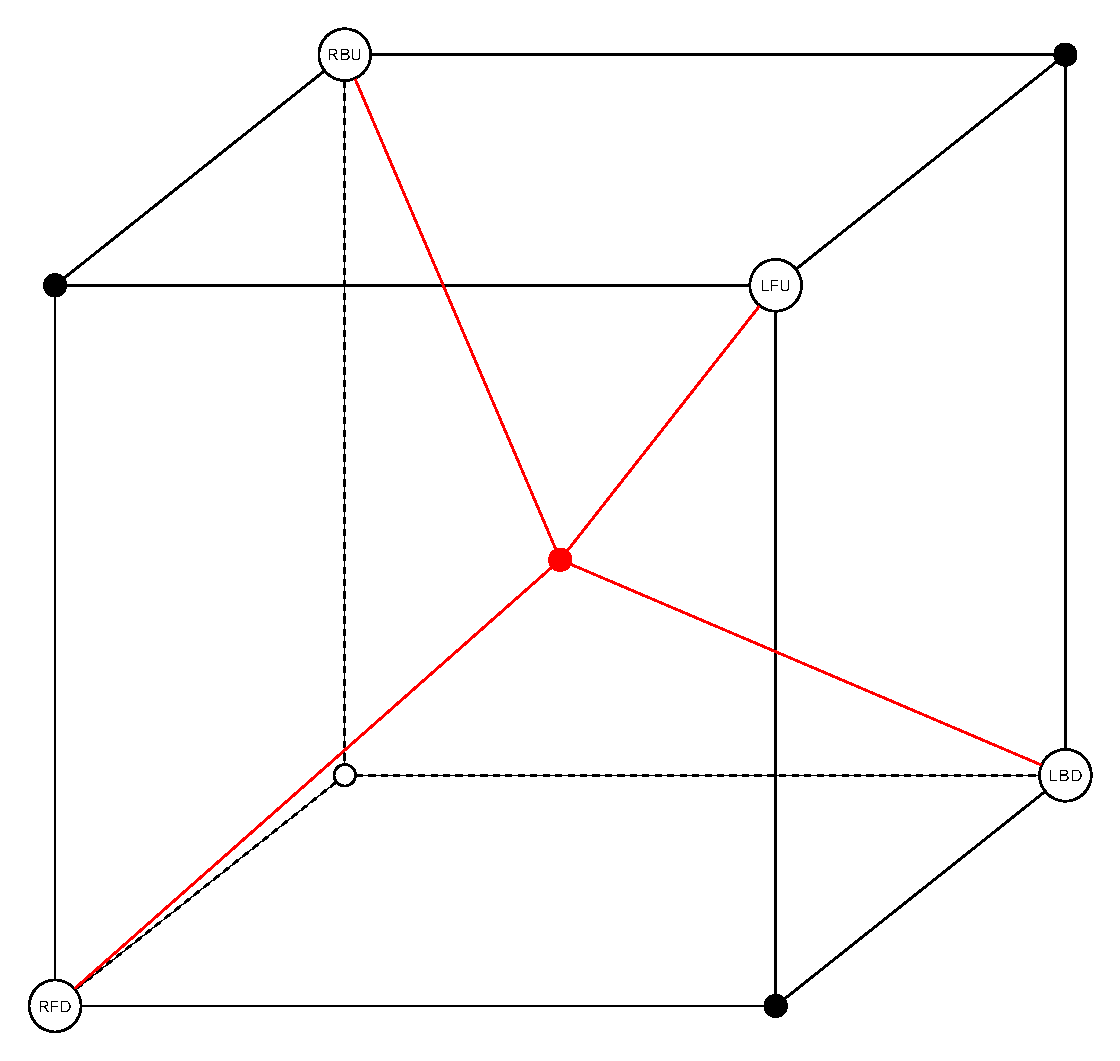
\includegraphics[width=.45\columnwidth]{tetrarec-cube}} \quad
%\subfloat[Spazio Tetraedrico]
%{\label{fig:tetracube}%
%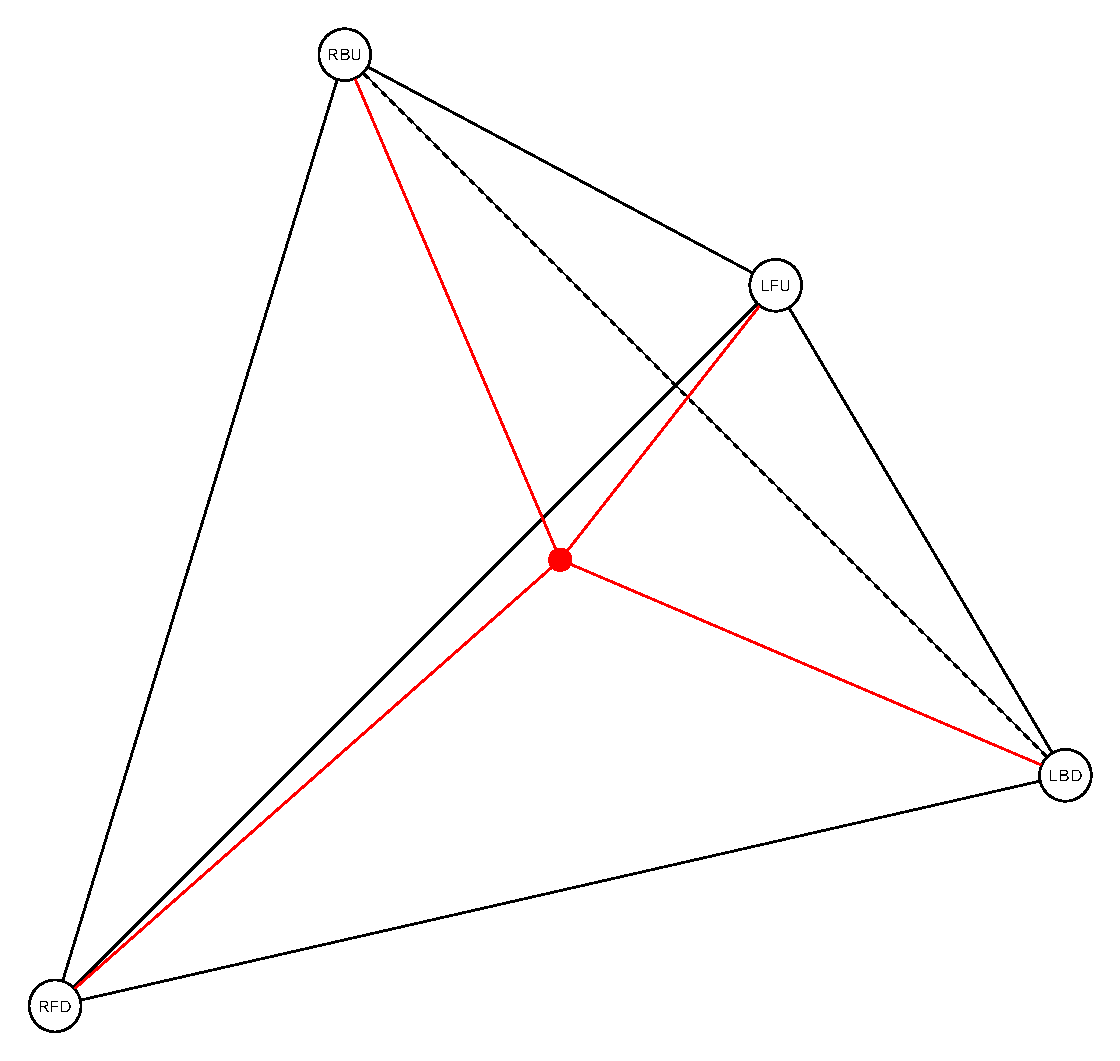
\includegraphics[width=.45\columnwidth]{tetrarec-tetrahedron}} \\
%\caption[Spazio Tetraedrico]{Spazio Tetraedrico}
%\label{fig:tetratetra}
%\end{figure}

%discorso riverbero non come elaborazione dell'amplificazione ma come costruzione delle
%riflesioni ambientali. Le distanze hai 4 stone identisci cosi da dislocare gli altoparlanti
%facilmente. Posto simmetrico posto. Filmarmonica in

\section{Riverberi}

Nel descrivere il percorso di ricerca applicata allo spazio espressa in questa
tesi si può definire il duplice ruolo \emph{strutturale} del riverbero:

\begin{description}
	\item [riverbero \emph{struttura-architettonica}]
		come definizione dell'ambiente, custodia del rito e della pratica musicale;
	\item [riverbero \emph{struttura-musicale}]
		come descrizione di un ambiente, custodia dell'idea musicale, culla di risonanze
		ricercate nella scrittura, forzate nei gesti, particelle del rito celato nel tubo
		sonoro e nel suo sconfinamento architettonico.
\end{description}

Qui i riverberi architettonici, siano essi locali che generali, non acquisiscono funzione di elaborazione
di un suono amplificato. L'altoparlante non ha funzione di amplificazione ma di dimensionamento della forma
acustica della chiesa. C'è una dimensione spaziale di creazione, di sintesi e simbiosi acustica con lo strumento
che non assume mai funzione di elaborazione ma dialogo, relazione e riflessione.

La riflessione, qualità intrinseca del riverbero, è oggetto di analisi e sintesi poli-dimensionale. 

In un dialogo tra il muro architettonico virtuale e la sola voce acustica dello strumento,
nel territorio mono-dimensionale di un confronto con la diffusione elettroacustica
convenzionale, si rischierebbe la scissione dall'immagine riflessa.

\clearpage

Il rapporto-confronto tra la voce acustica dello strumento musicale e la polifonica reazione 
architettonica al canto deve poter essere descritta nello spazio come un elemento simultaneamente
\emph{poli-dimensionale} e \emph{tempo-variabile}. Solo in questo modo ci si può permettere
di collocare le due entità, ormai voci dello stesso canto, in due luoghi diversi
della sala da concerto ed ottenerne un unico e solido corpo sonoro, mosso e stazionario così
come nella nella culla dell'ambiente originario. 

\begin{figure}[h]
\centering
{\includegraphics[width=.99\columnwidth]{ASM-IMG_3663}}
\caption[S. Luca, POV]{S. Luca, POV}
\label{fig:slucapov}
\end{figure}

La tecnologia elettroacustica è sussidio e consapevolezza di messa in scena funzionale alla
rievocazione del rito-luogo. La scelta del sistema elettroacustico \emph{S.T.ONE}\footnote{\emph{Spherical
Tetrahedral ONE}, diffusore elettroacustico composto di quattro facce triangolari per la riproduzione omni-direzionale
del campo sonoro} diviene elemento attivo nella stesura del brano sottoponendo elementi di dialogo strutturale, al tempo stesso
architettonico e musicale.

La scelta del numero minimo di diffusori, quattro, è volta alla ricerca della relazione di equilibrio tra
minima definizione tridimensionale e resa acustica in regime di verosimiglianza. Lo stesso Michael Gerzon
identifica in tre le sorgenti per la descrizione planare e quattro per la descizione perifonica.
Su questo principio si è operata una divisione dello spazio acustico descritto dalle mura in quattro regioni facilmente 
replicabili o identificabili in sala da concerto.

\section{Sistemi Elettroacustici}

Il progetto \emph{S.T.ONE} nasce dall'esigenza di poter eseguire musica elettroacustica,
sfruttando lo spazio sonoro creato dal mezzo elettronico, con caratteristiche percettive
acustiche analoghe a quelle degli strumenti tradizionali.

Un altoparlante tradizionale può essere controllato nella sola dimensione dinamica della
potenza e agendo su essa si può cercare un equilibrio con gli strumenti acustici.
Ma gli strumenti acustici hanno un comportamento molto più complesso, che implica relazioni
tra il fattore dinamico e quello timbrico e sopratutto spaziale del suono, creando uno
scollamento inevitabile tra ascolto acustico ed elettroacustico. S.T.ONE è il frutto di
una ricerca mirata alla soluzione di questo problema permettendo performance live in cui
la fusione tra i due soggetti, acustico ed elettroacustico, è totale, poli-dimensionale e completamente nuova all'ascoltatore. 

Con il diffusore S.T.ONE si può controllare la propagazione del suono riprodotto in tutte
le direzioni dello spazio e permettere di integrare questo controllo nei parametri della
composizione elettroacustica in un rapporto dialettico con lo strumento acustico.

L'ambizione è quella di superare un certo limite, identificato come appartenere intrinsecamente
all'oggetto altoparlante. L'oggetto, in quanto tale è stato il mezzo per giungere a quel limite e superarlo.

Il Limite. In un contesto di musica elettroacustica, ovvero di musica che si avvale parimenti
di oggetti acustici, strumenti tradizionali, oggetti elettrici ed elettronici, la diffusione
riprodotta dei suoni (mediante altoparlanti) ha sempre rappresentato un tema cruciale,
centrale per l'equilibrio acustico e musicale. Una buona integrazione tra suoni acustici
e suoni elettroacustici può tenere alta l'illusione di un unicum (ammesso che esso sia l'obiettivo)
ma è anche il varco attraverso cui introdurre il tarlo che farà crollare tutta la costruzione.
Questo ruolo di instabile funzionalità è si parametrabile all'ingegno che lo regola e lo dispone,
ma è anche dovuto al suo più grande limite: la direzionalità.

Un altoparlante nel migliore dei casi è un ottimo riproduttore di timbro e dinamica.
Ma l'elettroacustica ci ha insegnato che i parametri in gioco nella descrizione e
produzione di suono sono anche altri. La direzionalità, se vuole essere un parametro descrittivo,
deve poter variare nel tempo e non solo nella direzione di chi ascolta.

\vfill

\begin{figure}[h]
\centering
{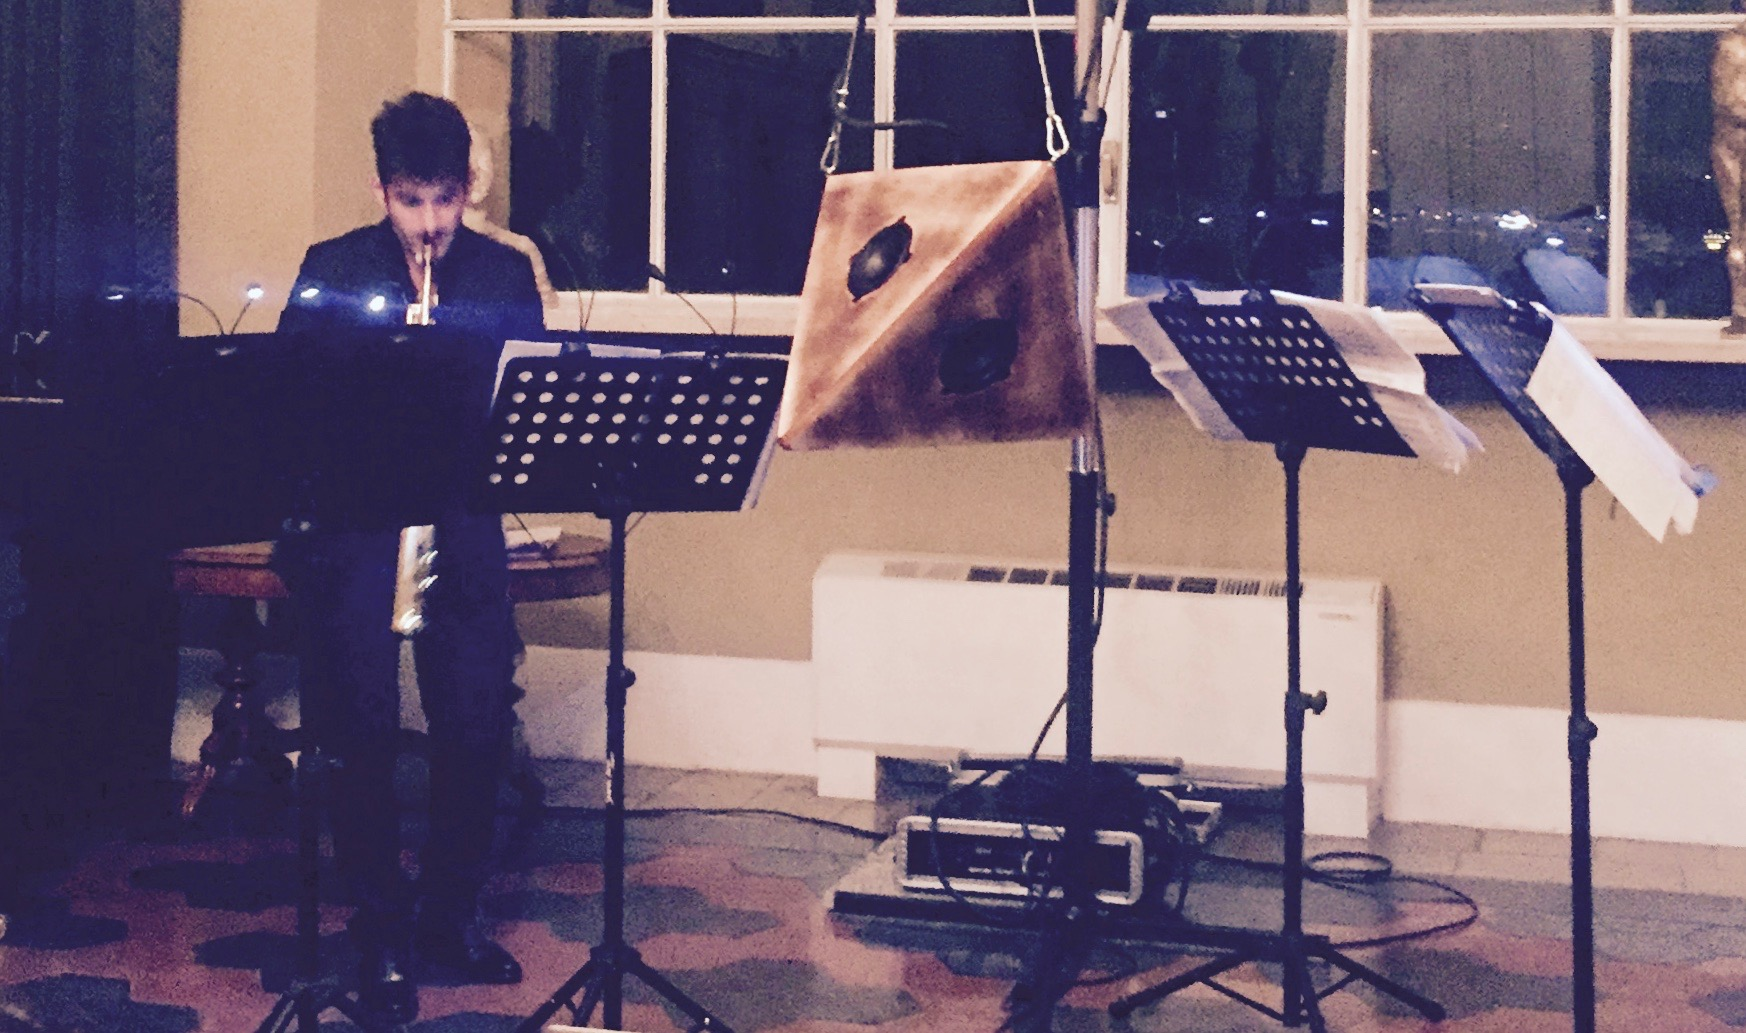
\includegraphics[width=.99\columnwidth]{IMG_3529}}
\caption[Danilo Perticaro. \emph{S.T.ONE}.]{Danilo Perticaro. \emph{S.T.ONE}.}
\label{fig:dpstone}
\end{figure}

% !TEX encoding = UTF-8
% !TEX TS-program = pdflatex
% !TEX root = ../Tesi.tex
% !TEX spellcheck = it-IT

%************************************************
\chapter{Acustica di san Luca: ricostruzione e perdita}
\label{cap:acustica}
%************************************************

%\begin{flushright}{\slshape
%  una citazione} \\ \medskip
%    --- un tizio
%\end{flushright}

~
\vfill

Nel processo di scelta ed elaborazione del materiale sonoro volto alla costruzione del brano,
mi è subito apparso ovvio intraprendere il cammino partendo non tanto dalle qualità timbriche
del sassofono o dall'astratta struttura e forma del brano, quanto dalle qualità intrinseche
del luogo come La chiesa di San Luca e Martina.

L'analisi di questo sistema acustico è incentrato nella sua ricostruzione tridimensionale,
virtualizzazione delle sue componenti, successivamente stratificate alla sala da concerto,
assieme alla registrazione dell'environment: anche per quest'ultimo sarà posto l'accento
sulla possibile riproduzione tridimensionale.

\begin{figure}[h]
\centering
{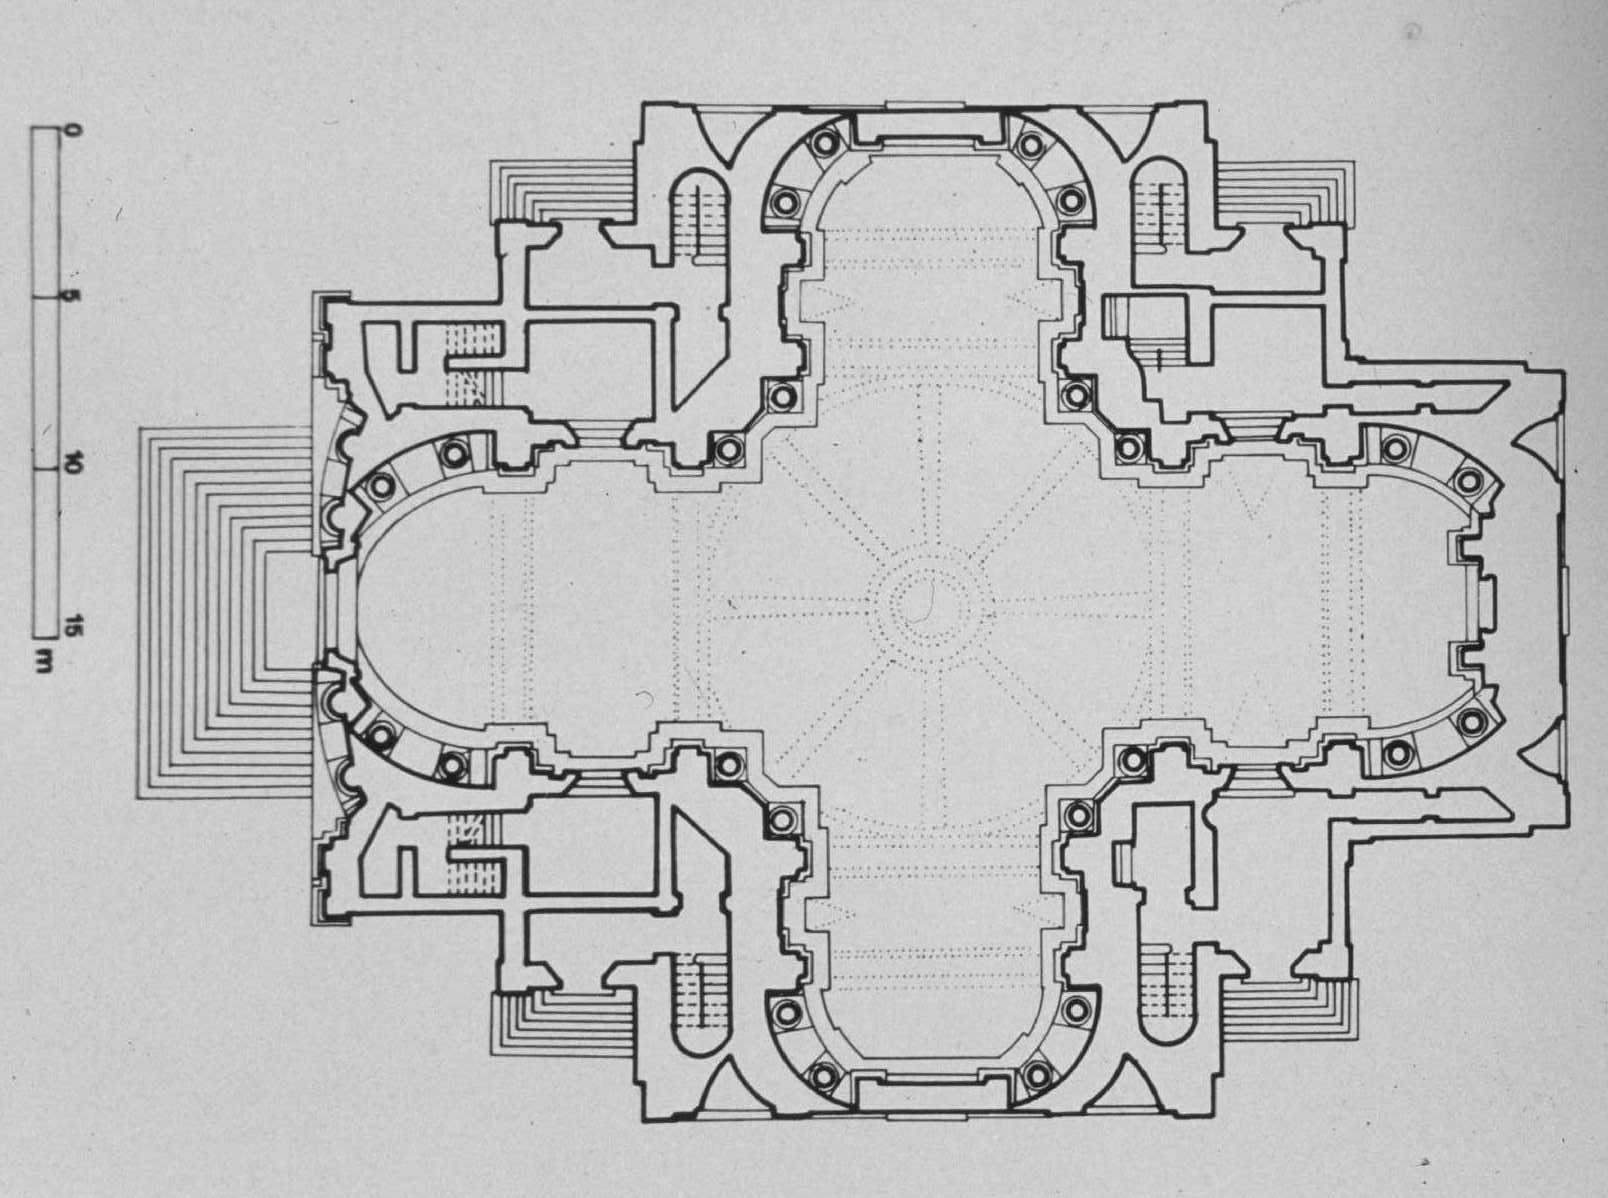
\includegraphics[width=.99\columnwidth]{04-Luca-Martina-pianta.jpg}}
\caption[Pianta S. Luca]{Pianta S. Luca}
\label{fig:tetratetra}
\end{figure}

\clearpage

\section{Cenno storico - scientifico}
\label{sec:storico}

Progettata nel 1635 da Pietro Berrettini da Cortona, la chiesa è composta da un unitaria
pianta cruciforme, che poggia sul titolo primitivo di Santa Martina, fondata nel VII
secolo da papa Onorio I, frontale all'arco di Settimio Severo. 

I due luoghi comunicano tramite il lucernario di Santa Martina e la scelta  di portare sopra
di esso l'altoparlante per l'indagine acustica, riguarda anche la ripresa delle riflessioni 
che avvengono nella chiesa inferiore e modificano l'ambiente sovrastante.
Per quanto riguarda i materiali è stato fatto affidamento alle fonti trovate all'accademia
di San Luca, nell'ipotesi di un nuovo sopralluogo e determinare, in base alle percentuali
di materiale nelle varie sezioni della chiesa il relativo livello di assorbimento della
chiesa e i conseguenti tempi delle prime  riflessioni

Materiali preponderanti della chiesa:

\begin{itemize}
	\item mattoni cotto
	\item marmo
\end{itemize}

I fenomeni principali acustici che vengono posti all'analisi riguardano:

\begin{enumerate}
	\item[a)] \textbf{il campo libero}, ovvero la distanza tra lo strumento/sorgente e gli ascoltatori. 
Stiamo parlando del confronto con il suono diretto e recepito dall'ascoltatore. Possiamo calcolarlo come:

\begin{equation}
I_{direct} = \frac{QW_{source}}{4\pi r^2}
\end{equation}

	\begin{description}
		\item[$I$] = intensità del suono diretto calcolato in watts per $m2$
		\item[$Q$] = direzionalità della sorgente 
		\item[$W$] = potenza della sorgente calcolata in watt 
		\item[$r$] = Distanza in $m^2$
	\end{description}
		
	\item[b)] \textbf{il campo riverberante}, ovvero l'energia successiva a quella diretta; prime riflessioni e coda.

\end{enumerate}

Ricordiamo che le prime riflessioni differiscono dal suono diretto sia per tempo (circa $80ms$) che direzione:


\begin{quoting}
The amount of energy, or power, removed by a given area of absorbing material will depend on the energy,
or power, per unit area striking it. As the sound intensity is a measure of the power per unit area this
means that the intensity of the sound reflected is reduced in proportion to the absorption
coefficient%\footcite{howjamie:acu}
\end{quoting}

importante è anche sottolineare come i materiali descritti in precedenza siano analizzati e ricondotti ad
una misurazione della riflessione “regionale”, specifica ai punti del quadrato, raccogliendo informazioni
riguardo alle differenti future risposte registrate.

Le mappe, descritte successivamente, riconducono a scelte di preparazione date dalla conformazione della
prima sala ove sarà eseguito il brano per la prima volta. Il sassofonista si trovava ad una
distanza di circa la metà dei metri cui sono stati disposti i microfoni per catturare le  riflessioni dello spazio.	

Il riverbero e le riflessioni della stanza sono il nostro argomento principale, ma l'analisi vedrà solo
l'attuazione di determinati punti sonori in regime e non tutta la pianta.
Schroeder a questo proposito spiega come %[DA SCRIVERE MEGLIO misura del ltempo di riverbero p. 15 /farina]
è possibile ricavare il tempo di decadimento (T60) tramite integrale della risposta all'impulso.

\begin{figure}
\centering
{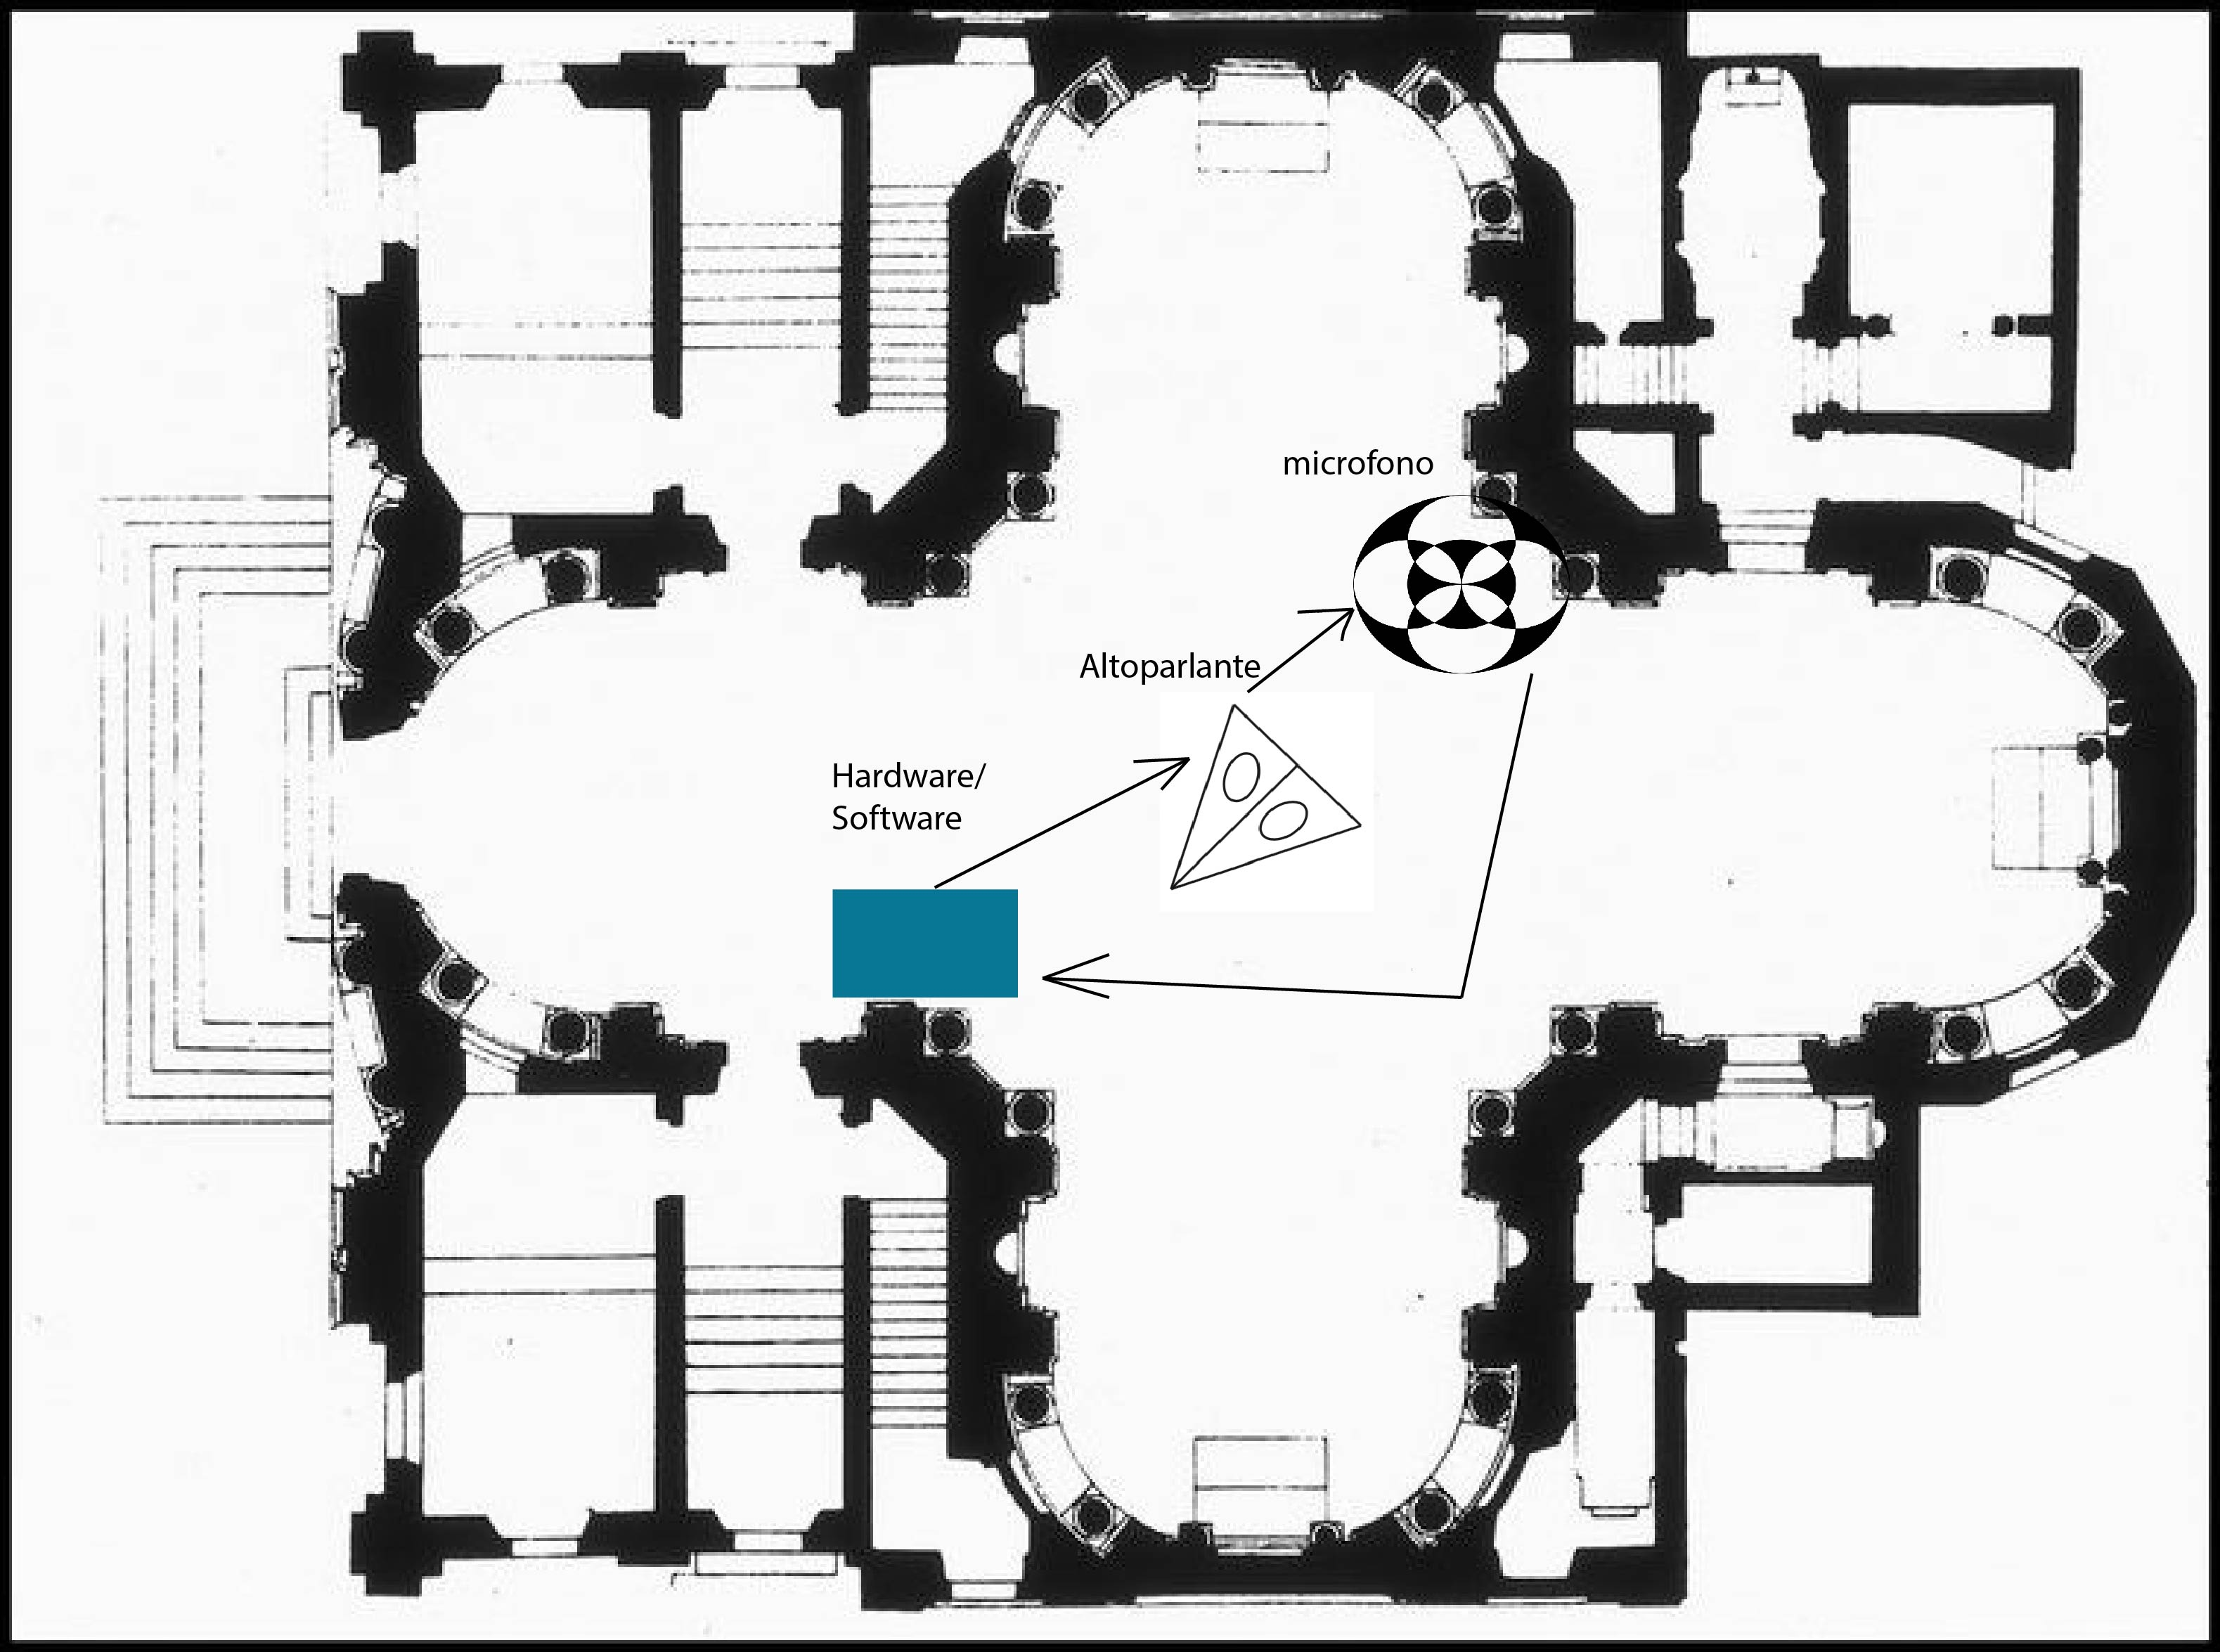
\includegraphics[width=.99\columnwidth]{file0031.jpg}}
\caption[Pianta S. Luca]{Catena di misurazione della risposta all'impulso}
\label{fig:tetratetra}
\end{figure}

\section{Risposta all'impulso}

Nel postulare le formule del nostro sistema lineare tempo invariante [LTI], Sabine ci rammenta
che questo sistema fisico  non deve  modificarsi nel momento di attuazione dell'analisi acustica.
L'LTI può essere rappresentato tramite una risposta all'impulso, ovvero misurare il suo
comportamento acustico.  Una sorgente, (nel nostro caso omnidirezionale) emette un
segnale $x(t)$  cui sarà sottoposto a modifiche del sistema:

dove

\begin{description}
	\item[$x(t)$] = segnale sorgente 
	\item[$F(x(t))$] = funzione di trasferimento
	\item[$n(t)$] = rumore ambiente
\end{description}

il segnale sorgente sarà comunque alterato dal trasduttore e dal rumore di fondo della stanza $n(t)$.

\begin{quote}

La risposta all'impulso $h(\tau)$ è la risposta del sistema nell'ipotesi che la
sorgente sonora generi un segnale $x(\tau)$ particolare, ossia un solo impulso unitario,
preceduto e seguito da una infinità di zeri. Esso è chiamato funzione delta di \emph{Dirac}:\footnote{3 Ivi. p. 5} 

\end{quote}

\begin{equation}
\delta(t) = 0~\textbf{per}~t~\neq 0~~~~~\int_{-\infty}^{+\infty}~\delta(t)dt=1
\end{equation}


Possiamo parlare della nostra risposta in Frequenza $H(f)$ (funzione di trasferimento),
come la  trasformata di \emph{Fourier} di $h(t)$: il prodotto tra gli spettri di $x$ e $y$ in funzione della frequenza

\begin{equation}
Y(f)= X(f)*H(f) 
\end{equation}

La funzione $F$ è prodotto di convoluzione tra il segnale di input e la risposta all'impulso del sistema

\begin{equation}
h(t):y(t)= n(t) + x(t) x h(t)
\end{equation}


\section{Scelta di distribuzione della sorgente e del microfono}

La peculiarità del progetto è quella di usare  quattro diffusori tetraedrici nella sala
da concerto per ri-descrivere lo spazio sonoro.

Il complesso sonoro tridimensionale è registrato tramite il microfono \emph{a-format}
messo nei quattro angoli del quadrato con il diffusore omnidirezionale al centro del quadrato. 

\begin{figure}
\centering
{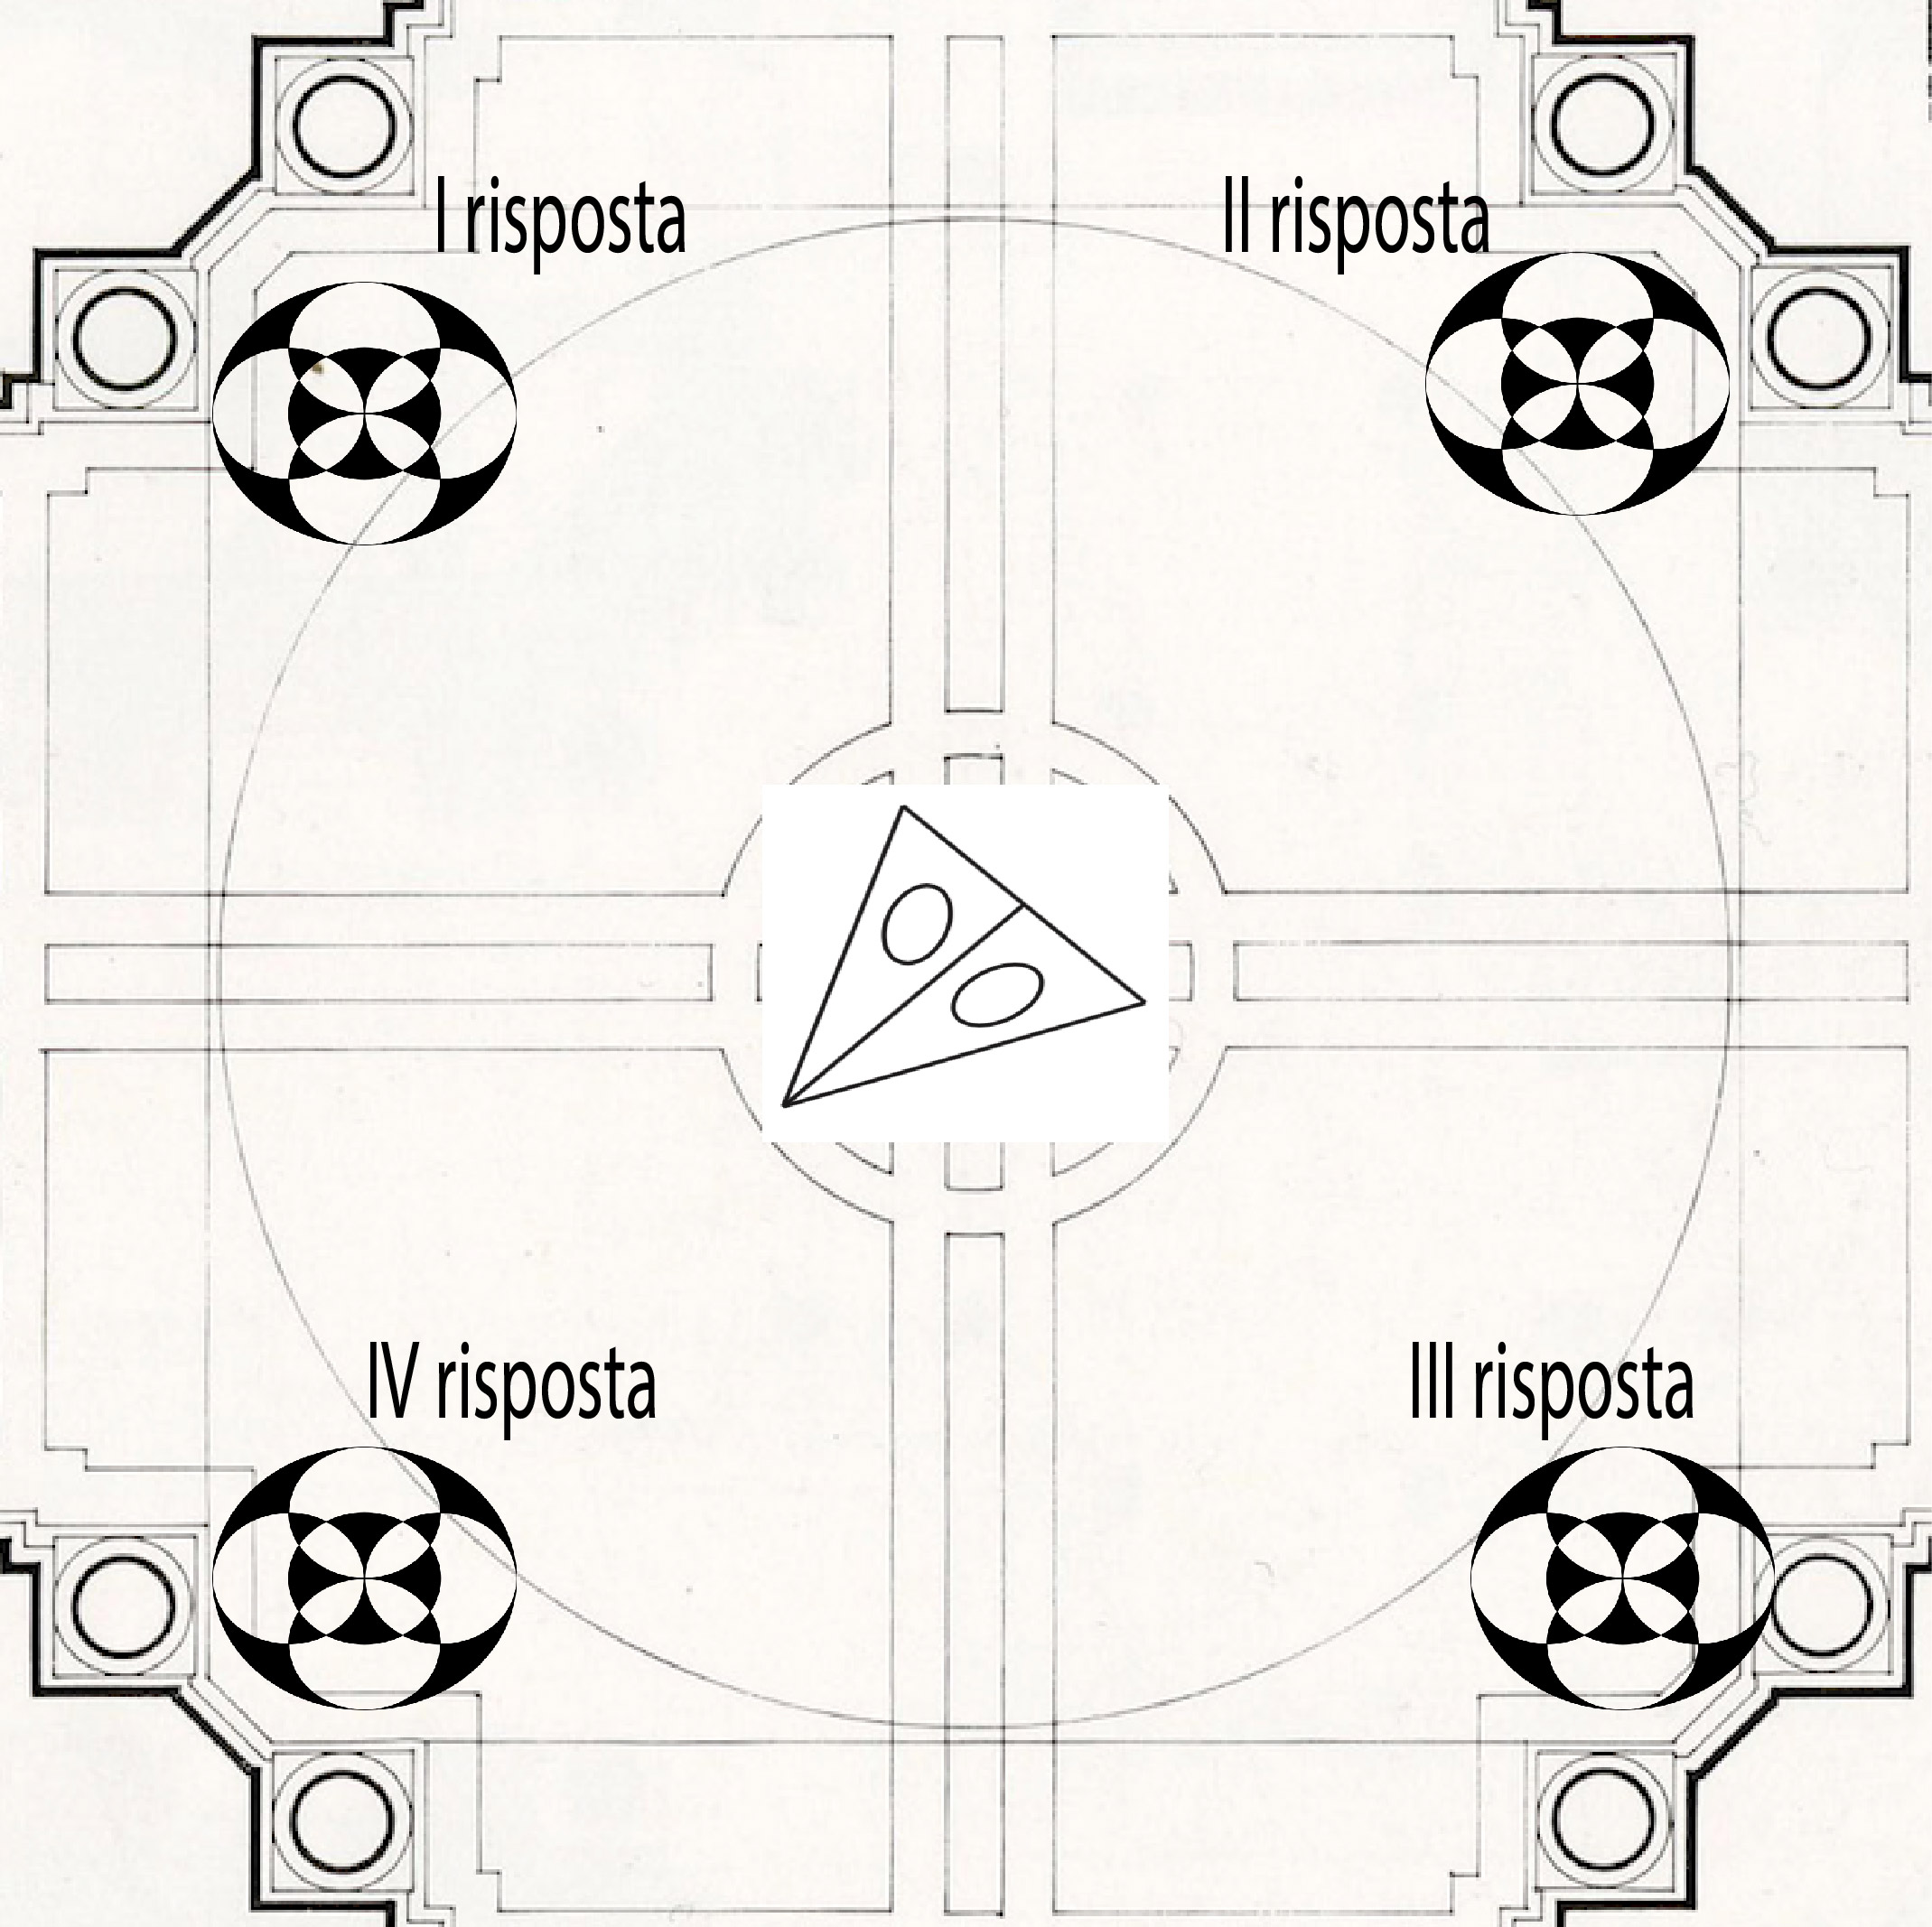
\includegraphics[width=.99\columnwidth]{file009.jpg}}
\caption[Pianta S. Luca]{Catena di misurazione della risposta all'impulso}
\label{fig:tetratetra}
\end{figure}

Le distanze sono state misurare ed equilibrate per dislocare i sistemi tetraedrici
facilmente nello spazio della sala.

\section{Strumentazione tecnica di misura}

La misurazione dell'ambiente ha fatto affidamento su questa strumentazione:

\begin{itemize}
	\item Mac Book pro portatile
	\item Finale di potenza t amp 700
	\item microfono A-format soundfield
	\item microfoni omni-direzionali dpa 4006
	\item microfoni omni-direzionali audio line OM1
	\item S.T.ONE
\end{itemize}

\section{Prova}

In un indagine di primo livello dall'acustica di San Luca è stato importante suonare
parte del brano con l'interprete all'interno della chiesa. Partendo da un concetto
di auralizzazione per poi via via affrancarsi dalla metodologia scientifica e ricavare
la propria risposta nell accoppiamento tra stanza virtuale e stanza reale, è stato
importante ricavare empiricamente le regioni che meglio soddisfavano le eseigenze
compositive. L'interprete ha eseguito parte del brano in diversi punti della navata,
portando all'attenzione le riflessioni e risonanze preponderanti. 
Le prove che hanno dato maggior riscontro acustico in funzione musicale riguardano
il centro della chiesa e la collanna di sinistra vicina al cenacolo.

la scelta di posizionamento del sistema tetraedrico interno alla chiesa per la
risposta all'impulso si è basata anche per il posizionamento possibile del sassofonista
in concerto.
Un possibile quadrante che inglobi il pubblico in concerto, corrispondente al
quadrante interno alla croce, dove sono ubicati i banchi da chiesa.
Come nel posizionamento dello STone per la risposta all'impulso, sono state
effettuate molteplici prove per sistemare per il quadrante ottimale. Di seguito
le configurazioni accettate per l'esecuzione:

\begin{figure}[h]
\centering
\subfloat[Asia personas duo]
{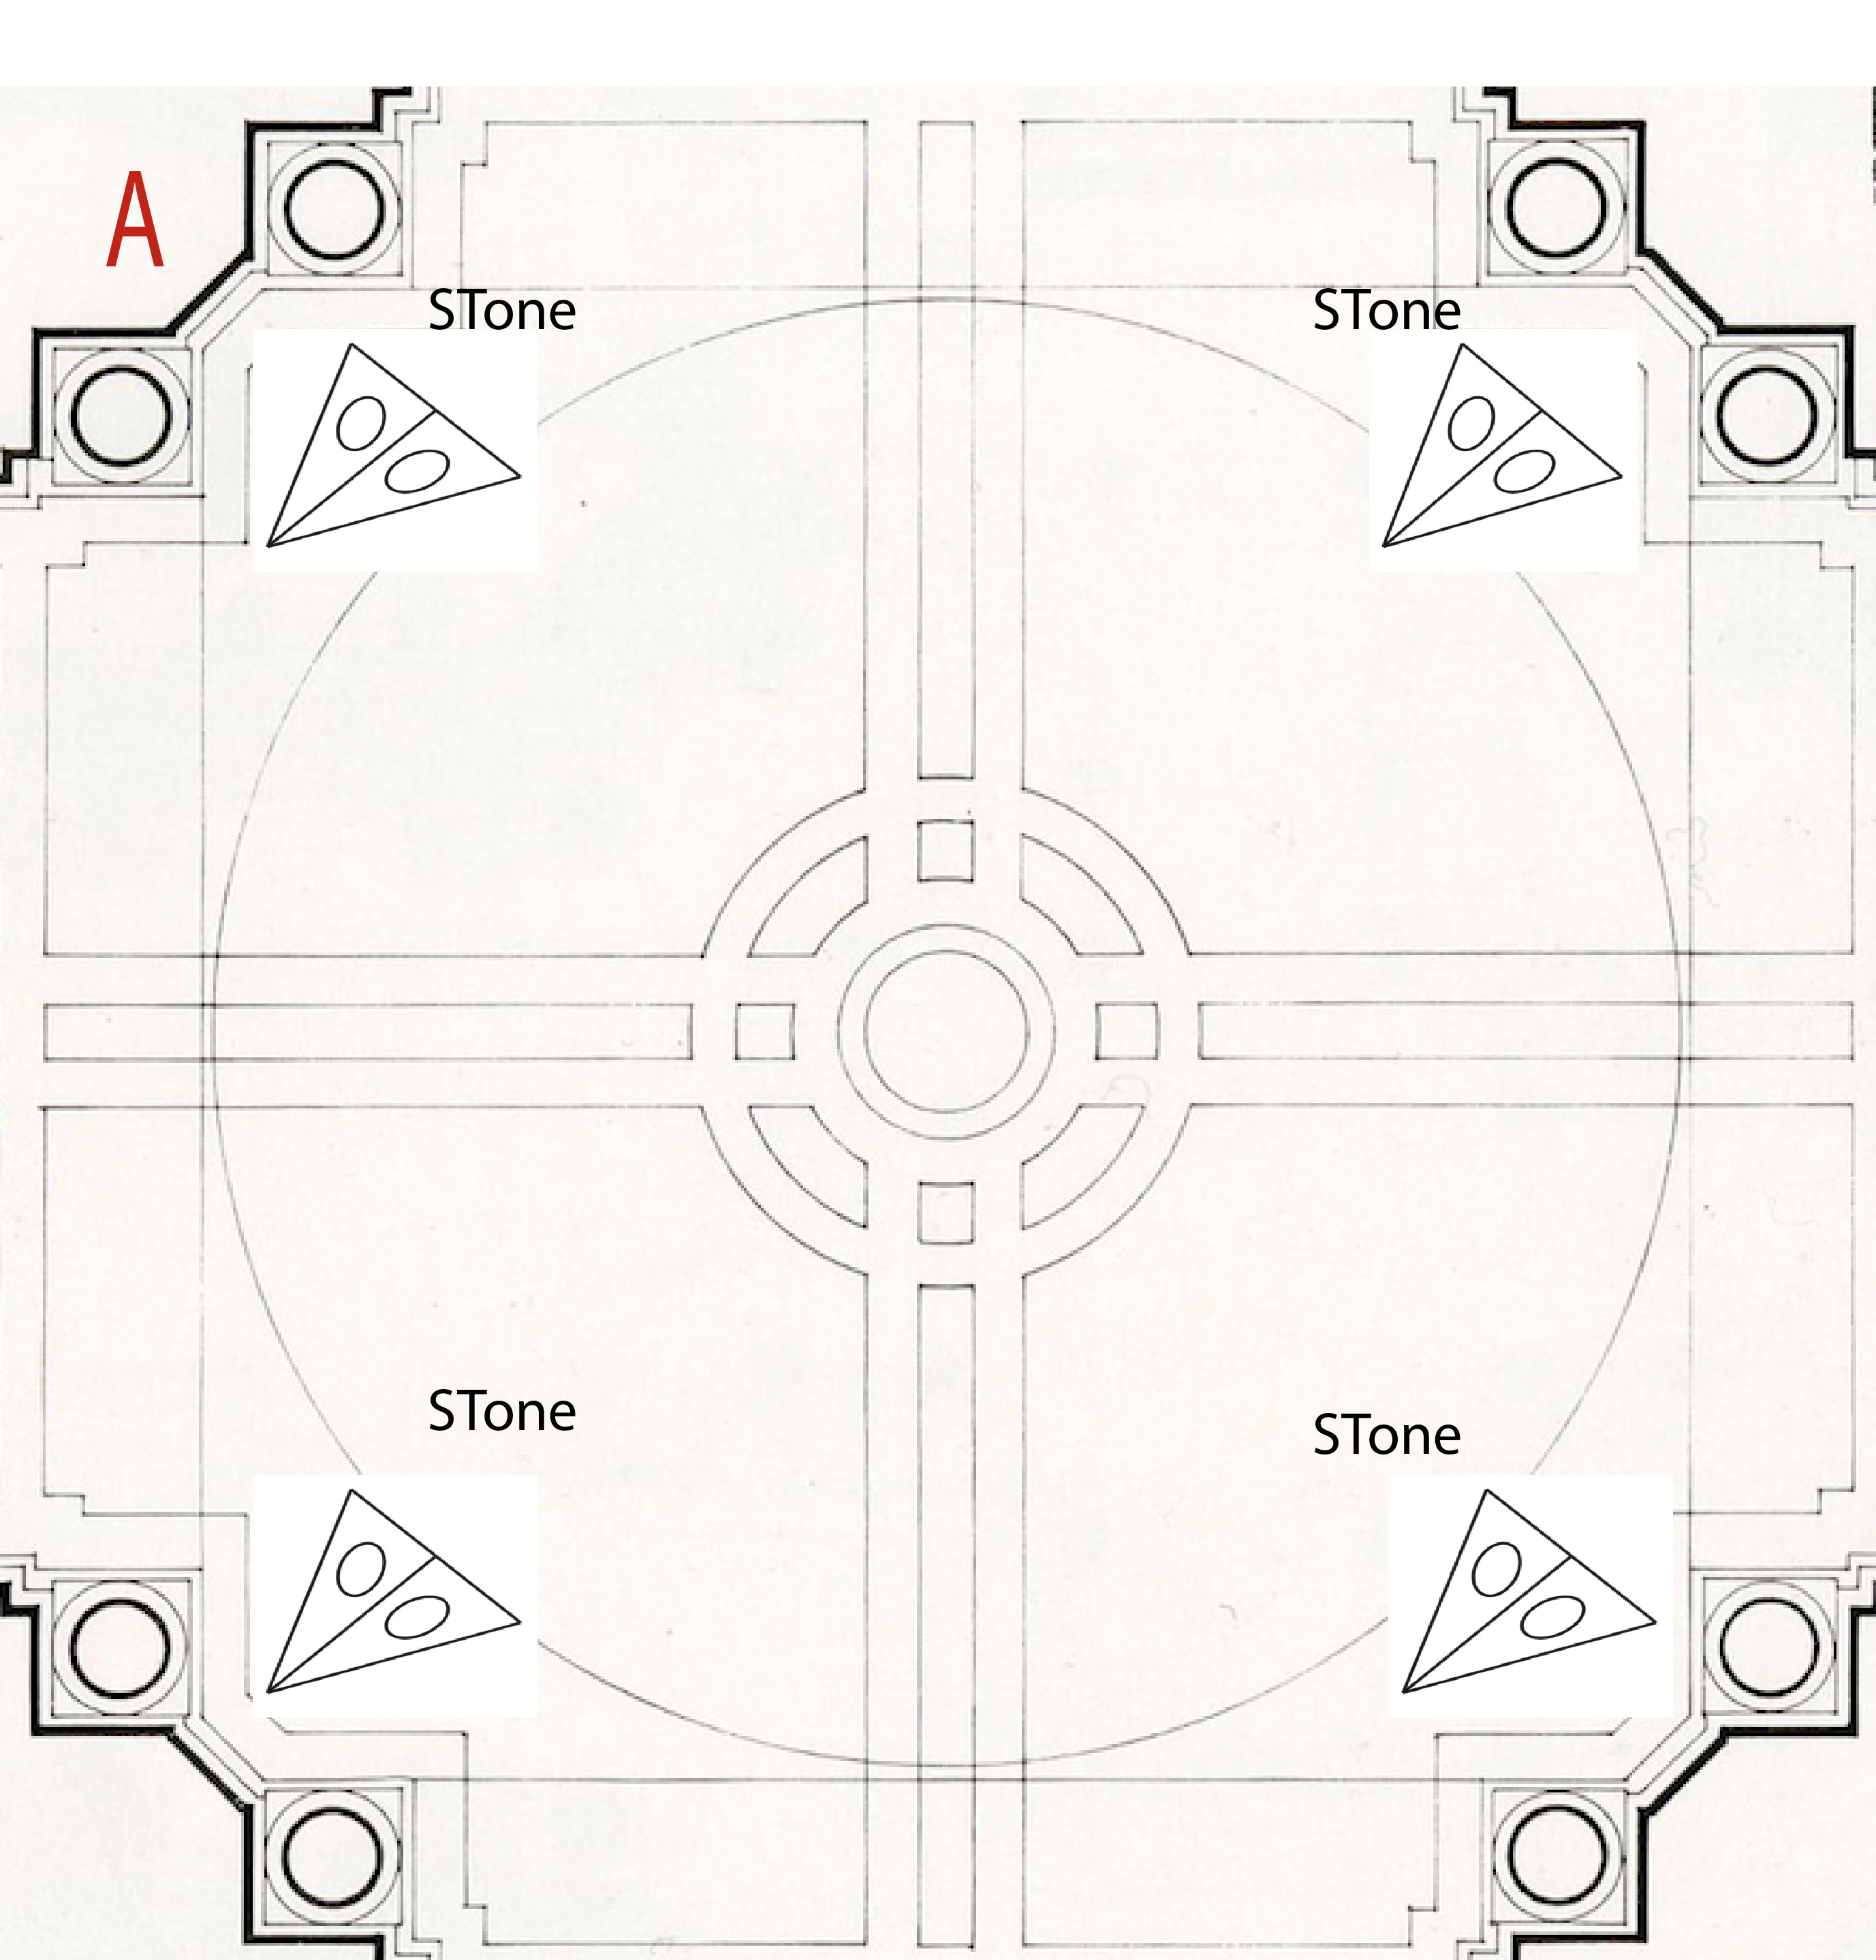
\includegraphics[width=.45\columnwidth]{file004.jpg}} \quad
\subfloat[Pan ma signo]
{\label{fig:example-b}%
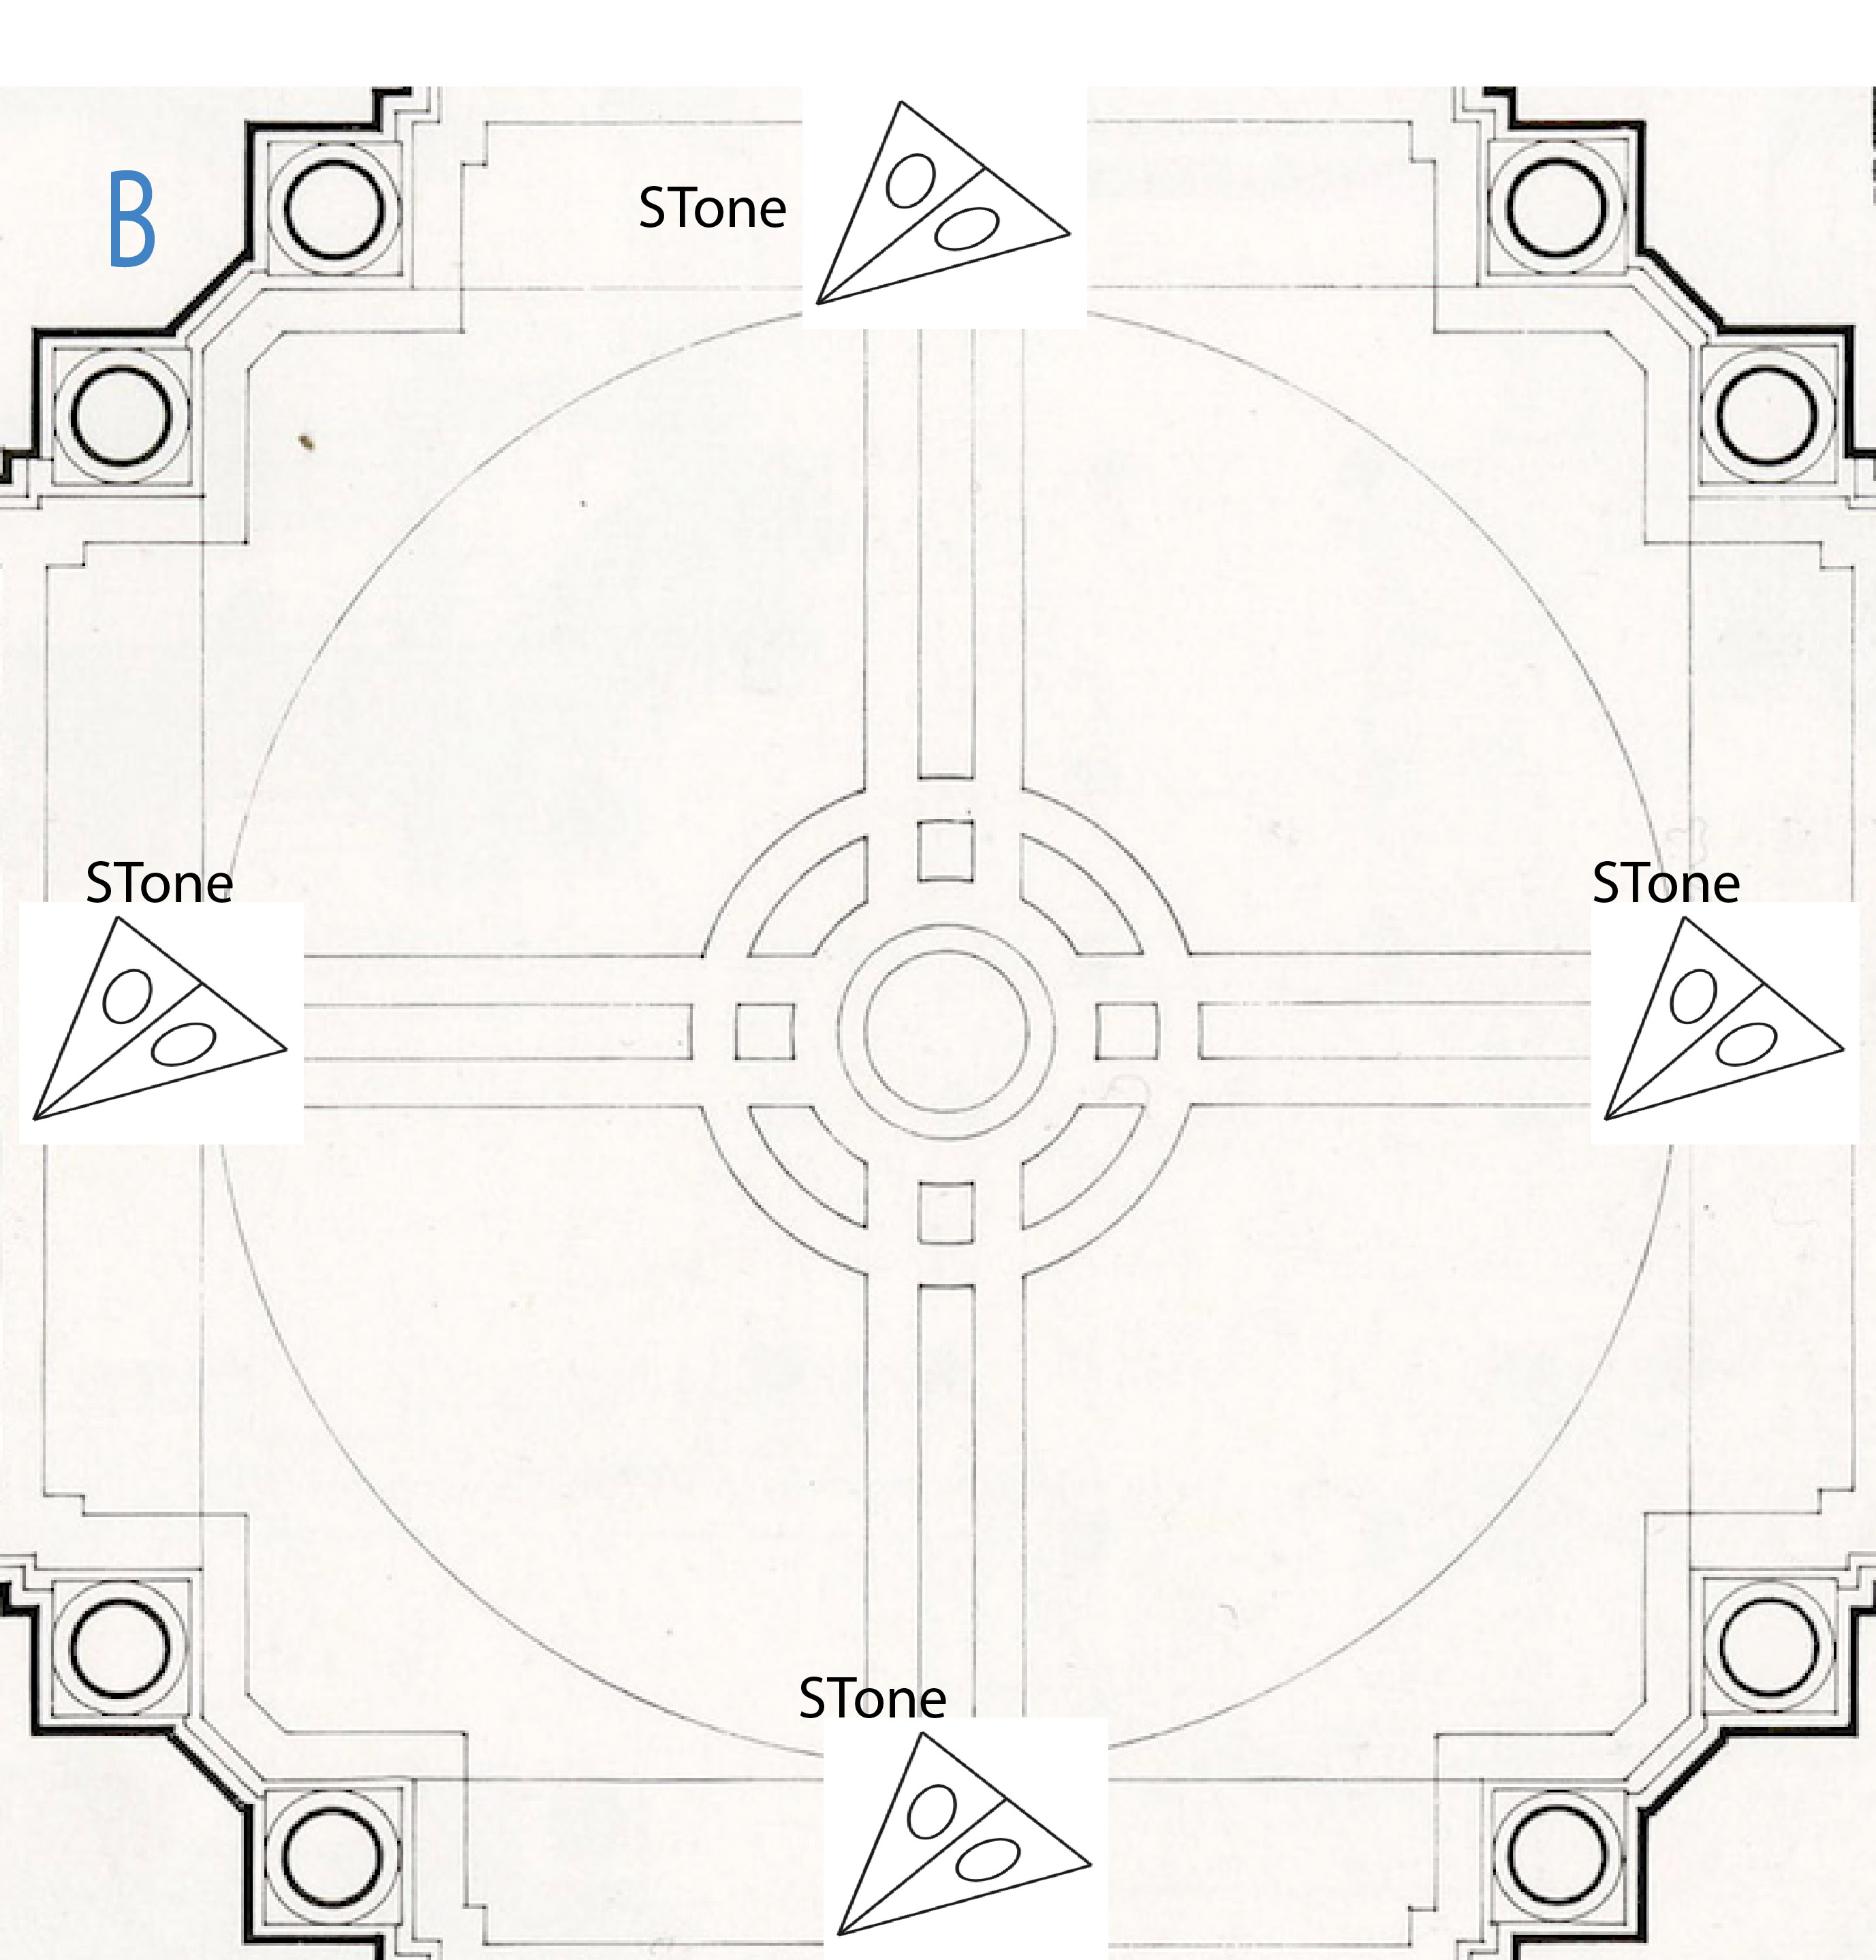
\includegraphics[width=.45\columnwidth]{file005.jpg}}
\end{figure}

La prima esecuzione prevista per il brano è stata alla Filarmonica Romana il
22/11/2016 e la conformazione della sala è un rettangolo: Questo ha escluso
la configurazione B di tipo "diamond" in quanto avremmo avuto l'interprete in
prospettiva dell'altoparlante e il ridimensionamento del quadrante formato dagli
Stone inscritto,rispetto alla configurazione A che non presentava questo tipo di inconveniente.

\section{Impulse Response Retrieval} 

La tecnica di misurazione adottata fa affidamento al descrittore acustico di tipo ESS.
Essendo la chiesa vicino ad un via molto trafficata e con possibilità di rumore di
fondo molto alta, si era pensato di determinare le caratteristiche dell'ambiente
tramite sistema MlS, maximum length sequences. 
Ricordiamo che questa tecnica mette in correlazione segnale di ingresso $ x(n) $
e segnale di uscita $ y(n) $ di un sistema lineare. 
In pratica si applica questa sequenza pseudocasuale (simile ad un rumore bianco)
all'ingresso del sistema e moltiplicando poi questo segnale in uscita con la
sequenza iniziale di ingresso. Il risultato è la funzione delta di Dirac:

Questa misurazione permette un ottimo bilanciamento suono/rumore di fondo,
anche in condizioni molto precarie.
Ma il metodo  di sweep (lineare o esponenziale che sia) permette un risulatato
migliore al fronte di distorsione armoniche del sistema (altoparlante).

Metodo ESS (exponential sine sweep)

Il nostro descrittore acustica è uno segnale sweep esponenziale, che si sviluppa nel tempo.
Partendo da una sequenza dal di sopra del dc. 
La frequenza si raddoppia ripetutamente a tempi di intervallo indentico.

Tempo ed energia sono spese per partire dalla bassa frequenza fino alle alte:

si è partiti da una frequenza di 30 HZ fino a 22000 HZ:
per partire a frequenze cosi basse è stato integrato un sub woofer.

A differenza di un chirp lineare si possono raccogliere maggiori informazioni selle frequenze percepite. 

EQUAZIONE \\
------file006-----

w1 frequenza di partenza normalizzata in radianti (frequenza angolare iniziale)

w2 è la frequenza di arrivo in radianti (frequenza angolare finale)

n è l'indice dei sample

n è il numero dei samples

Anche questo sistema porta con se, oltre all'effetto di riverbero della stanza anche
le componenti di rumore e gli effetti di distorsione non lineare di cui parlavamo in
precedenza (dirsione della fondamentale della componente elettronica)

Anche per quanto riguarda l'ampiezza il segnale è costante tutto il tempo. L'analisi
mostra un decay della magnitudine di 6 db per ottava. Questo decay della magnitudine
viene compensato quando la risposta all'impulso è calcolata tramite deconvoluzione,
in quanto la compensazione è fatta nel domnicio digitale e non altera il rapporto
segnale rumore favorendo la gamma di bassa frequenza del segnale di prova.

Vista la registrazione di molteplici risposte bisogna arrivare alla maggior efficenza
del sistema.
 Lo spettro registrato non risulta perfetto in quanto caratterizzato da frequenze di
 ripple agli estremi, che in taluni casi superano i + 5 db. I confini del chirp ( di start e di stop)
 presentano queste frequenze indesiderate, causa anche la parziale cancellazione di fase e somma sopra il segnale. 


chirp expo:2.5 further ripple reduction: fade-in window  e deconvoluzione

segnale di putput y(t)convoluto con il filtro inverso

risposte markidis


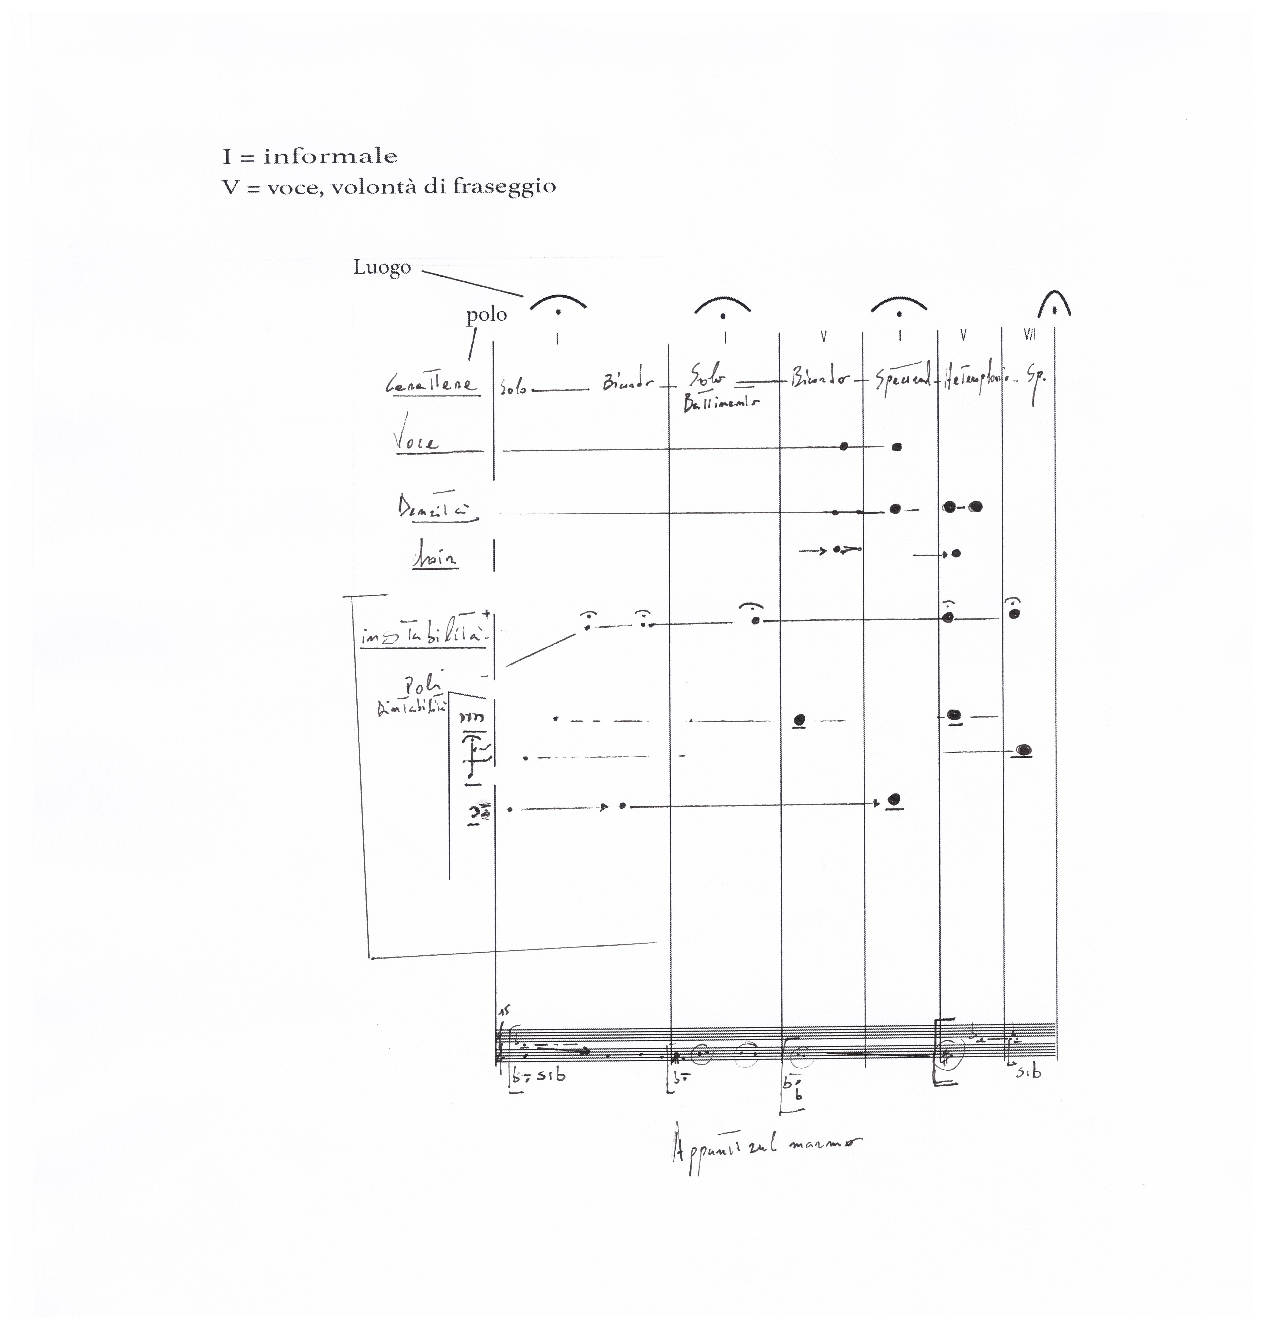
\includepdf[scale=1.3, offset=10 0]{macrostruttura.pdf}
% !TEX encoding = UTF-8
% !TEX TS-program = pdflatex
% !TEX root = ../Tesi.tex
% !TEX spellcheck = it-IT

%************************************************
\chapter{Acustica di san Luca: ricostruzione e perdita}
\label{cap:acustica}
%************************************************

%\begin{flushright}{\slshape
%  L'enigma che risuona dalle mascelli feroci della vergine \\
%  \medskip
%    --- Pindaro
%\end{flushright}

%-preludio e cenno storico
%
%-environment
%
%-struttura
%
%
Qui, l’incedere di una risonanza è legata ad un corpo/luogo, lentamente mutabile:
uno spazio che è memoria di superficie. Abitare questo ascolto è stato il primo
passo della scrittura, il formalizzarsi e il perdersi di una molteplice voce,
abitante abitato da \emph{per sempre}. 

La scelta del luogo, dello spazio d'ascolto è il punto di partenza.
Partenza (come dipartita), della stessa scrittura strumentale tradizionale. 
Lo studio dello spazio di San Luca ha instaurato diverse relazioni che
congiungono i diversi strati di elaborazione, dalla macro alla micro-struttura.
%
%
%
%
%
\section{Coscienza di scrittura}

L'immemorialit à dell'evento scandisce sia il gesto formale che la struttura,
organizzando i contributi qualitativi del suono e la loro distribuzione
temporale e spaziale. Immemorialità dello stesso suono come strumento trasformato
e non riconducibile a:

Altezza temperata.

È volutamente ricercato nello strumento la sua oscillazione  attorno a dei
poli frequenziali (descritti successivamente), cercando la massima <<instabilità-controllata>>.
Giochi di oscillazione che intercorrono tra l’evidente parametro multifonico e la sua de-costruzione timbrica.
Lo stesso vale per i battimenti, altri importanti operatori di trasformazione.


-----fileA------



\section{Modalità di emissione omogenea}

Gradazioni controllate di soffio e suono, oltre che intonazione di aberrazioni prodotte tramite saliva e spostamento dell'imboccatura.     

\begin{figure}
\centering
{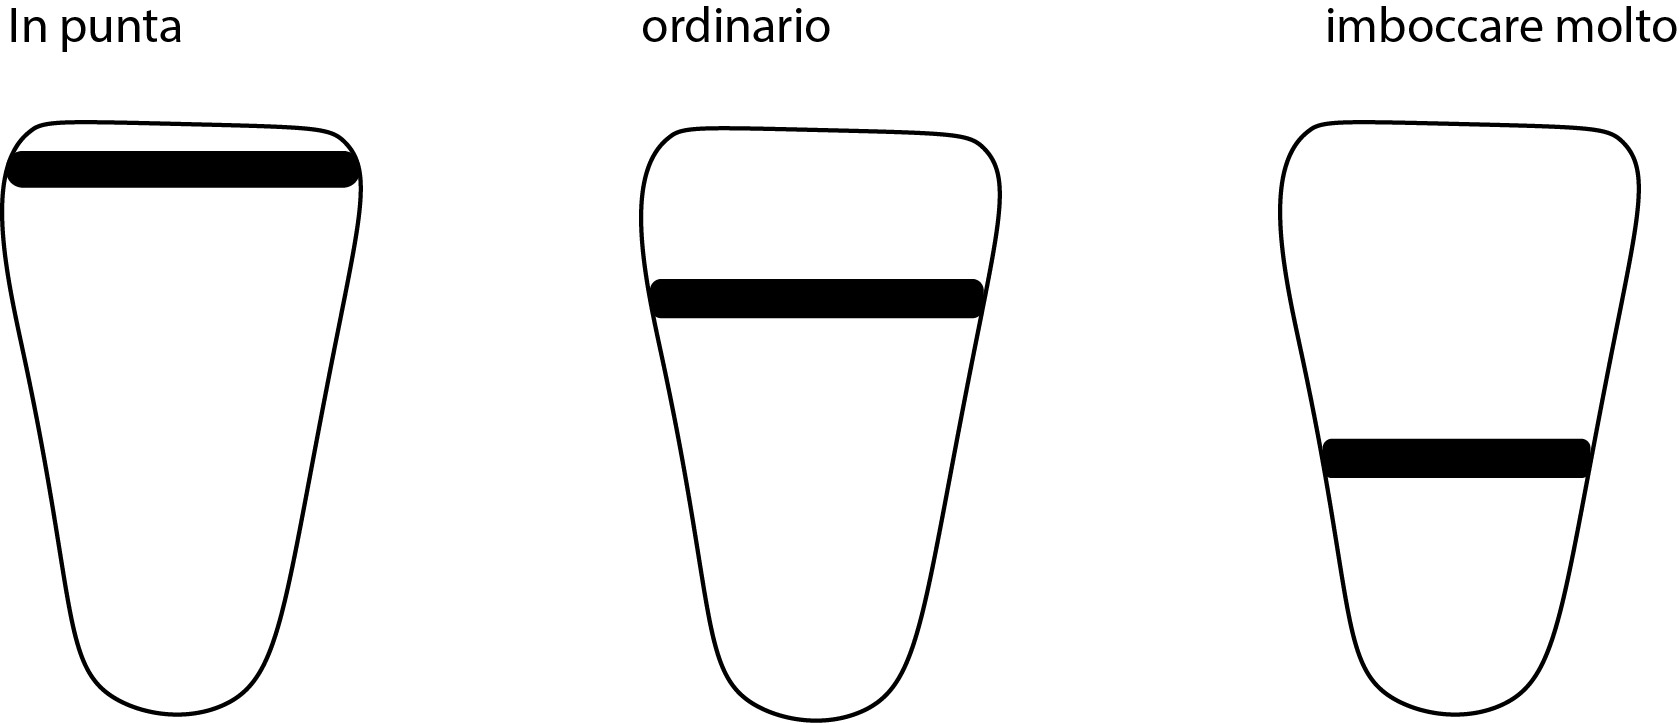
\includegraphics[width=.65\columnwidth]{sax_boc.jpg}}
\caption[Pianta S. Luca]{Schemi imboccatura}
\label{fig:tetratetra}
\end{figure}

Perché il sassofono?

Le caratteristiche cercate in questo strumento si basano sulla possibilità
di insistere su determinati fattori; il corpo/bocca dello strumentista, 
le modifiche della colonna armonica, i suoi armonici sovracuti, doppiati
e triplicati nel medesimo tempo/istante.
Il sassofono soprano rende possibile la continua modulazione tra multifonici:
una “corrente continua”,  dove il movimento lento (pensato assieme all'impronta
elettronica del luogo) permette lo stazionamento di determinate parziali
e il passaggio fluido tra differenti bicordi. È stato fondamentale lo studio
dei parziali multifonici, il loro isolamento monodico e la possibilità di 
“entrare” ed “uscire” dalla posizione di generazione multifonica.

Possiamo dividere le qualità di queste parziali in famiglie:

disegnino1* = parziali <<treshold tones>>  -  
disegnino2 = <<shadow sound>>: suoni che non possono essere i solati.
È stato posto l’accento sulle possibili aberrazioni che si pongono su ottave differenti
rispetto al suono cardine, rendendo il contenuto spettrale più instabile e ricco.
disegnino3 = instabile : alcune regioni frequenziali di multifonici presentano una
difficile risposta. Battimenti o parziali sovracuti avranno una risposta non lineare.
Si deve tendere a cercare una sorta di <<modulazione di ampiezza>>. Cercare il suono.
* i simboli sono presi dal trattato di Weiss e Netti



-----fileC-----



Conseguenziale a questo tipo di scrittura il  rapporto e la pratica con lo strumentista.
Le tecniche estese di partenza vengono dagli studi di Weiss e Netti,ma il percorso di
elaborazione, di nuova scoperta di emissione e modulazione di timbro e altezze è
stato condotto assieme al sassofonista Danilo Perticaro.

[[[[[a specchio da una parte le Qualità sonore da l'altra i suoni cardine]]]]]

Qualità sonore e trasformazione suoni cardine del brano\footnote{Alcune delle transizioni
e multifonici non si trovano nel brano. Gli schemi preparatori riportano anche lavoro a
monte rispetto allo studio con lo strumentista.  Provandoli successivamente ci siamo
resi conti di incongruenze legate alla difficolta di diteggiatura o differente
legatura di emissione (dinamiche eccessivamente differenti portavano ad non legare le posizioni)}
Ogni diteggiatura nel suo legarsi presenta un effetto di modifica non solo 
frequenziale ma dello spettro stesso delle parziali.

Assottigliamento verso i suoni sovracuti del sassofono(materiale povero spettralmente)

fileD
 
frequenza ambigua che interpola

Emissione - soffio - battimento
 
 
schema microstruttura con modifica del suono:

file E

fondamentale -parziale accrescimento-svuotamento

la logica d'uso di queste tecniche si pone lontana dagli schematismi di "effetto" che ruotano attorno all'articolazione di note.                                      

\section{Environment}

La logica spaziale proposta con la risposta all'impulso e la riproduzione tramite sistema tetraedrico, ha portato a concepire un uso delle fonti sonore che gravitano interne e all’esterno dell'ambiente della chiesa di San Luca.
 La registrazione e la riproduzione tramite sistema A-format permetteva di delineare una cartografia tridimensionale degli eventi: tramite un'azione musicale preparata sono stati controllati e scanditi i materiali suonati all'interno della chiesa: preparata in quanto si vuole nascondere il più possibile l’evento acustico dalla percezione familiare, dal suo effettivo sguardo <<concreto>>.
La logica di registrazione segue il quadrante interno alla chiesa utilizzato per gli impulsi.

\subsection{struttura del nastro}

Note 

Tre esecutori                                                            
la durata del nastro è di circa 10 minuti.
è da considerare ad libitum. Sarà chiuso il processo da parte del regista del suono.
L'incontro con la parte strumentale è fortemente aleatoria. Environment attorno all’ascoltatore, attorno allo strumentista,con un range medio-grave. È possibile riscrivere il nastro partendo dai materiali e dallo schema relativo alle dinamiche generale. Il tutto deve essere tra <<pppppp>> e <<pp>>. Mai s

MATERIALI

A= ambiente esterno alla chiesa [controllare adeguatamente il livello d'ingresso del soundfield]
B= banchi da chiesa (scricchiolio)
C= sedie
D= passi
E= voci




\subsection{Schema}

La scelta di preparare  dal vivo il materiale  concreto e non elaborarlo successivamente
è dato dal fatto che i 4 tape registrati dal soundfield potevano andare incontro a
sfasamenti togliendo la componente tridimensionale. Solo tagli e riposizionanamenti
del nastro, fade in e fade out delle tracce.

Sono state registrate due azioni con una configurazione dei microfoni diversa,
per poi essere integrati nell'esecuzione:

quadrante A            +             quadrante b


Come si vede dallo schema la tridimensionalità del nastro è prevista solo per i relativi STone:
in questo caso solo quelli anteriori, paralleli alla posizione dello strumentista.
Su gli altri 2 STone è prevista diffusione omnidirezionale.

Schema di tracce mandate agli STone

La discesa come struttura.

Il tragitto costruito tramite il sassofono soprano è direttamente intrecciato alle sue
possibilità più remote, ad uno studio acustico che insiste sulla transizione di bicordi.
Un passaggio da un certo grado intervallare a l’altro, in una continua trasformazione, 
pronta ad dilatarsi in un tempo immobile. Questo gioco, del perdersi e riprendersi
variando nei registri e nelle  qualità vibrazionali, mette in relazione luoghi
acustici eterogenei dalla ricca complessità timbrica.
Luogo,scrittura, concepito nelle possibilità che ogni passo, gradazione nata dal
primo bicordo di sesta minore, poteva mettere in gioco: l’individuazione del successivo
istante e cambio di frequenze è circoscritto alle posizioni di chiave appena precedute.
Il successivo bicordo è in molti dei casi costituito da una delle parziali che fa da
ponte tra un intervallo e l altro. 
Questa successione di eventi (rizoma tra due voci poste ora in accordo poi battimento)
è il fondamento della struttura, dell’alveare polifonico e microtonale.
Le tecniche estese consentono di sfruttare parziali inarmoniche, tipiche di questo
strumento, organizzando dei poli microtonali. 

Prendo in esempio l’evento generante che gravita attorno alla frequenza del sib5.

Il successivo movimento tiene conto di questo polo alterando l’intervallo a favore
di un spostamento quartitonale, per poi riassumere nei succesivi movimenti l’aspetto originario:

È comunque da tenere conto che i microtoni non sono pensati su una scala temperata ma in cent. 
Possiamo prendere come intervalli polari/ circostanziali:

sesta minore/quinta aumentata/—————seconda minore/battimento 

La qualità del battimento è fondamentale e questa trasformazione entro la seconda minore.

Esso è “interruttore” per lo spostamento del polo.

Il progetto di queste polarità frequenziali è andato di pari passo con quella di
relazioni alla costruzione di qualità descritte in precedenza.   

\subsection{Klangqualitatemelodie}

variazioni delle qualità attorno a i poli. tipo di variazione 

operatori di instabilità

variazione informale









  



%\input{Capitoli/03-appunti}
%% !TEX encoding = UTF-8
% !TEX TS-program = pdflatex
% !TEX root = ../Tesi.tex
% !TEX spellcheck = it-IT

%************************************************
\chapter{Ipsum}
\label{cap:ipsum}
%************************************************

\lipsum[1]

\section{Lorem}
\lipsum[2]

\section{Ipsum}
\lipsum[3]

\section{Dolor}
\lipsum[4-5]
%\appendix
%% !TEX encoding = UTF-8
% !TEX TS-program = pdflatex
% !TEX root = ../Articolo.tex
% !TEX spellcheck = it-IT

%************************************************
\section{Dolor}
\label{sec:dolor}
%************************************************

\lipsum[1]

\subsection{Mane}
\lipsum[2]

\subsection{Tekel}
\lipsum[3]

\subsection{Fares}
\lipsum[4-5]

% *****************************************************************
% Materiale finale
%******************************************************************
%% !TEX encoding = UTF-8
% !TEX TS-program = pdflatex
% !TEX root = ../CME-III-ARTICOLO.tex
% !TEX spellcheck = it-IT

%*******************************************************
% Bibliografia
%*******************************************************
\nocite{*}
\printbibliography
%% !TEX encoding = UTF-8
% !TEX TS-program = pdflatex
% !TEX root = ../Tesi.tex
% !TEX spellcheck = it-IT

%*******************************************************
% Dichiarazione
%*******************************************************
\cleardoublepage
\phantomsection
\pdfbookmark{Dichiarazione}{Dichiarazione}
\chapter*{Dichiarazione}
\thispagestyle{empty}

Lorem ipsum dolor sit amet, consectetuer adipiscing elit. Ut purus elit, vestibulum ut, placerat ac, adipiscing vitae, felis. Curabitur dictum gravida mauris. Nam arcu libero, nonummy eget, consectetuer id, vulputate a, magna. Donec vehicula augue eu neque.

Pellentesque habitant morbi tristique senectus et netus et malesuada fames ac turpis egestas. Mauris ut leo. Cras viverra metus rhoncus sem. Nulla et lectus vestibulum urna fringilla ultrices.

\bigskip
 
\noindent\textit{\myLocation, \MakeTextLowercase{\myTime}}

\smallskip

\begin{flushright}
    \begin{tabular}{m{5cm}}
        \\ \hline
        \centering\myName \\
    \end{tabular}
\end{flushright}

\end{document}





